% !TEX root = ../my-thesis.tex
%
\chapter{Introduction to Bayesian Inference}
\label{sec:bayes}
\cleanchapterquote{A picture is worth a thousand words. An interface is worth a thousand pictures.}{Ben Shneiderman}{(Professor for Computer Science)} \\
Bayesian Inference is a method of statistical inference that uses Bayes' theorem to update the probability of a hypothesis as more data are observed or more information becomes available. It is an essential technique in mathematical statistics and the polar opposite of the frequentist approach, which makes predictions based solely on data from an experiment. In the Bayesian approach a \textit{prior} distribution $p\left(\pmb{\theta}, \sigma^2\right)$ is introduced as part of the model. This distribution is intended to express a state of knowledge or ignorance about $\pmb{\theta}$ and $\sigma^2$ prior to obtaining the data. Using the prior distribution, the likelihood function $p\left(\pmb{x}|\pmb{\theta},\sigma^2\right)$, and the observed data $x$, it is possible to calculate the probability distribution $p\left(\pmb{\theta},\sigma^2\right|\pmb{x})$ of $\pmb{\theta}$ and $\sigma^2$ given the data $\pmb{x}$. This distribution is called the \textit{posterior} distribution of $\pmb{\theta}$ and $\sigma^2$ an is used to make inferences about the parameters\autocite[Cf.][]{box2011bayesian}.
\section{Preliminaries}
This work follows strict notation rules to easily represent different elements such as matrices or graphs and contains frequently used abbreviations. These and some other basic concepts used in this work are introduced below. The notation follows the one used by Rue and Held\autocite[Cf.][]{rue2005gaussian}.
\subsubsection*{Matrices and Vectors}
Vectors and matrices are indicated by bold notation, such as $\pmb{x}$ and $\pmb{A}$. The transpose of $\pmb{A}$ is denoted by $\pmb{A}^T$. The element in the \textit{i}th row and \textit{j}th column of $\pmb{A}$ is referenced by $A_{ij}$. This notation is also used for vectors and $x_i$ denotes the \textit{i}th element of a vector. The vector $\left(x_1,x_{i+1},...,x_j\right)^T$ is abbreviated to $\pmb{x}_{i:j}$. If the columns $\pmb{A}_1, \pmb{A}_2,...,\pmb{A}_m$ of a $n\times m$ matrix $\pmb{A}$ are stacked on top of each other, this is denoted by $\hbox{vec}\left(\pmb{A}\right)=\left(\pmb{A}_1^T,\pmb{A}_2^2,...,\pmb{A}_m^T\right)$. Deleting rows and/or columns from $\pmb{A}$ creates a \textit{submatrix}. If a submatrix of a $n\times n$ matrix $\pmb{A}$ can be obtained by removing rows and columns of the same index, it is called a \textit{principal submatrix}. If this matrix can be obtained by deleting the last $n-r$ rows and columns, it is called a \textit{leading principal submatrix} of \pmb{A}. \\
A diagonal $n\times n$ matrix $\pmb{A}$ is denoted by $\hbox{diag}\left(\pmb{A}\right)$ and has the following structure:
\begin{equation*}
    \hbox{diag}\left(\pmb{A}\right)=\begin{pmatrix}
    A_{11} \\
    & \ddots \\
    &&A_{nn}
    \end{pmatrix}.
\end{equation*}
The identity matrix is denoted by $\pmb{I}$. \\
If $A_{ij}=0$ for $i>j$ or $A_{ij} = 0$ where $i>j$, then $\pmb{A}$ is called \textit{upper triangular} and \textit{lower triangular} respectively. The \textit{bandwidth} of a matrix $\pmb{A}$ is defined as $\max\left\lbrace|i-j|:A_{ij}\neq0\right\rbrace$. The \textit{lower bandwidth} is given by $\max\lbrace|i-j|:A_{ij}\neq $ $0\hbox{ and } i > j\rbrace$. $|\pmb{A}|$ denotes the \textit{determinant} of a $n\times n$ matrix $\pmb{A}$ and is equal to the product of the eigenvalues of $\pmb{A}$. The \textit{rank} of $\pmb{A}$, referenced by $\hbox{rank}\left(\pmb{A}\right)$, is the number of linearly independent rows or columns of $\pmb{A}$. The sum of the diagonal elements is called \textit{trace} of $\pmb{A}$, $\hbox{trace}\left(\pmb{A}\right)=\sum_{i}A_{ii}$.\\
Finally, '$\odot$' denotes the element-wise multiplication of two matrices of size $n\times m$, '$\oslash$' denotes the element-wise division and raising each element of a matrix $\pmb{A}$ to a scalar power uses the symbol '$\owedge$'.
\subsubsection*{Lattice and Torus}
$\mathcal{I}_{\pmb{n}}$ denotes a (regular) \textbf{lattice} (or grid) of size $\pmb{n}=\left(n_1, n_2\right)$ (in the two-dimensional case). $\pmb{x}$ can take values on $\mathcal{I}_{\pmb{n}}$ and $x_{i,j}$ denotes the value of $\pmb{x}$ at location $ij$, for $i=1,...,n_1$ and $j=1,...,n_2$. For easier reading this will be shortened to $x_{ij}$. On an \textit{infinite lattice} $\mathcal{I}_{\pmb{\infty}}$, $ij$ are numbered as $i=0,\pm1,\pm2,...,$ and $j=0,\pm1,\pm2,...$. \\
A lattice with cyclic or toroidal boundary conditions is referred to as \textit{torus} and is denoted by $\mathcal{I}_{\pmb{\infty}}$. The dimension is $\pmb{n}=\left(n_1,n_2\right)$ (in the two-dimensional case) and all indices are modulus $\pmb{n}$ and run from 0 to $n_1-1$ or $n_2-1$. If a GMRF $\pmb{x}$ is defined on $\mathcal{I}_{\pmb{n}}$, the toroidal boundary conditions imply that $x_{-2,n_2}$ is equal to $x_{n_1-2,0}$ since $-2\mod n_1$ is equal to $n_1-2$ and $n_2\mod n_2$ is equal to 0.\\
An \textit{irregular lattice} refers to a spatial configuration of regions $i=1,...,n$ where the regions (mostly) have common boundaries, for instance the states of a nation.
\begin{figure}[H]
   \centering
       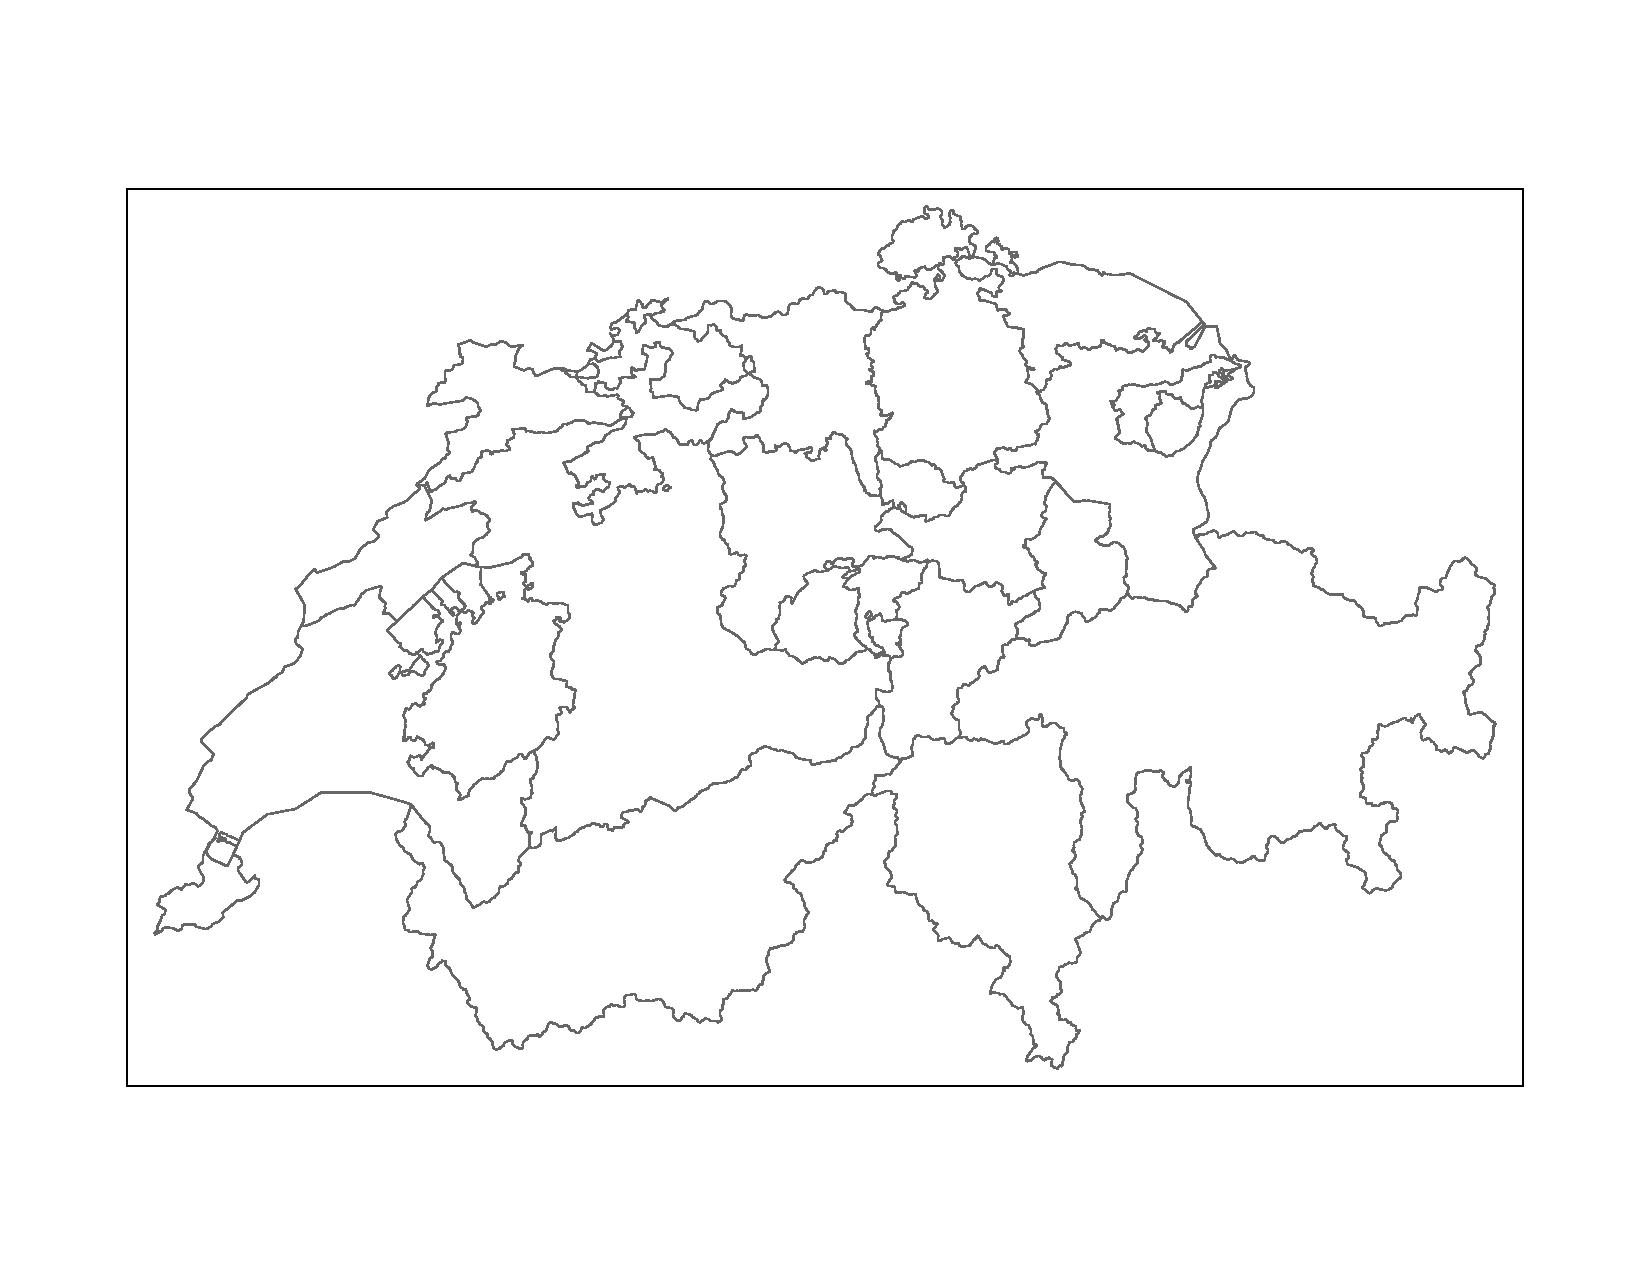
\includegraphics[page=1,width=.7\textwidth]{switzerland.pdf}
 \caption{The cantons of Switzerland, an example of an irregular lattice.}
 \label{fig:lattice}
\end{figure}
\subsubsection*{General Notation and Abbreviations}
For $C\in\mathcal{I}=\left\lbrace1,...,n\right\rbrace$ let $\pmb{x}_C=\left\lbrace x_i:i\in C\right\rbrace$. $-C$ denotes the set $\mathcal{I-C}$ such that $\pmb{x}_{-C}=\left\lbrace x_i:i\in C\right\rbrace$. For two sets $A$ and $B$, $A\setminus B=\left\lbrace i:i\in A \hbox{ and } i \notin B\right\rbrace$. \\
$\pi\left(\cdot\right)$ denotes the density of its arguments, for example $\pi\left(\pmb{x}\right)$ for the density of $\pmb{x}$ and $\pi\left(\pmb{x}_A|\pmb{x}_{-A}\right)$ for the conditional density of $\pmb{x}_A$, given $\pmb{x}_{-A}$. '$\sim$' is used when a variable is 'distributed' according to the law $\mathcal{L}$.  \\
The expected value is denoted by $\mathbb{E}\left[\cdot\right]$, the variance by $\hbox{Var}\left(\cdot\right)$, the covariance by $\hbox{Cov}\left(\cdot\right)$, the precision by $\hbox{Prec}\left(\cdot\right)=\hbox{Cov}\left(\cdot\right)^{-1}$, the correlation by $\hbox{Corr}\left(\cdot,\cdot\right)$ and a probability by $\mathbb{P}\left(\cdot\right)$.
\subsubsection*{Symmetric Positive Definite Matrices}
An $n \times n$ matrix $\pmb{A}$ is \textit{positive definite} exactly if
\begin{equation*}
    \pmb{x}^T\pmb{A}\pmb{x}>0,\hspace{20pt}\forall\pmb{x}\neq\pmb{0}.
\end{equation*}
If $\pmb{A}$ is also symmetric, it is called a symmetric positive definite (SPD) matrix. Only SPD matrices are considered and sometimes the notation '$\pmb{A}>0$' is used for an SPD matrix $\pmb{A}$. \\
An SPD matrix $\pmb{A}$ has some of the following properties.
\begin{itemize}
    \item[1.] $\hbox{rank}\left(\pmb{A}\right)=n$.
    \item[2.] $|\pmb{A}|>0$.
    \item[3.] $A_{ii}>0$.
    \item[4.] $A_{ii}A_{jj}-A_{ij}^2>0$, for $i\neq j$.
    \item[5.] $A_{ii} + A_{jj}-2|A_{ij}|>0$ for $i\neq j$.
    \item[6.] $\max A_{ii}>\max_{i\neq j}|A_{ij}|$.
    \item[7.] $\pmb{A}^{-1}$ is SPD.
    \item[8.] All principal submatrices of $\pmb{A}$ are SPD.
\end{itemize}
If $\pmb{A}$ and $\pmb{B}$ are SPD, $\pmb{A}+\pmb{B}$ is also SPD, but the reverse is generally not true. Additionally, if $\pmb{AB}=\pmb{BA}$, $\pmb{AB}$ is SPD. \\
The following conditions are all sufficient and necessary for a symmetric matrix $\pmb{A}$ to be SPD:
\begin{itemize}
    \item[1.] All eigenvalues $\lambda_1,...,\lambda_n$ of $\pmb{A}$ are strictly positive.
    \item[2.] There exists such a matrix $\pmb{C}$ that $\pmb{A}=\pmb{CC}^T$. If $\pmb{C}$ is lower triangle, it is called the \textit{Cholesky triangle} of $\pmb{A}$.
    \item[3.] All leading principal submatrices have strictly positive determinants.
\end{itemize}    
A sufficient, but not necessary condition for a (symmetrical) matrix to be SPD is the criterion of \textit{diagonal dominance}:
    \begin{equation*}
        A_{ii}-\sum_{j:j\neq i}|A_{ij}|>0,\hspace{20pt}\forall i.
    \end{equation*}
    A $n\times n$ matrix $\pmb{A}$ is called a \textit{symmetric positive semidefinite} (SPSD) matrix. An SPSD matrix $\pmb{A}$ is sometimes denoted '$\pmb{A}\geq0$'\autocite[Cf.][]{rue2005gaussian}.
\clearpage
\section{Basic Concepts of Bayesian Theory}
\subsection{Bayes' Theorem}
At the heart of Bayesian inference is \textit{Bayes' theorem}, which describes the probability of an event given prior knowledge of factors that might influence the event. \\
Let $\pmb{x}^T=\left(x_1,...,x_n\right)$ be a vector of $n$ observations whose probability distribution $p\left(\pmb{x}|\pmb{\theta}\right)$ depends on the values of $k$ parameters $\pmb{\theta}^T=\left(\theta_1,...,\theta_k\right)$. Let $p\left(\pmb{\theta}\right)$ be the probability distribution of $\pmb{\pmb{\theta}}$. Then 
\begin{equation}
    p\left(\pmb{x}|\pmb{\theta}\right)p\left(\pmb{\theta}\right)=p\left(\pmb{x},\pmb{\theta}\right) = p\left(\pmb{\theta}|\pmb{x}\right)p\left(\pmb{x}\right).
\end{equation}
Given the observed data $\pmb{x}$, the conditional distribution of $\pmb{\theta}$ is
\begin{equation}
    p\left(\pmb{\theta}|\pmb{x}\right)=\frac{\pmb{p}\left(\pmb{x}|\pmb{\theta}\right)p\left(\pmb{\theta}\right)}{p\left(\pmb{x}\right)}.
\end{equation}
This last statement is known as Bayes' theorem. The \textit{prior} distribution $p\left(\pmb{\theta}\right)$ contains knowledge about $\pmb{\theta}$ without knowledge of the data. $p\left(\pmb{\theta}|\pmb{x}\right)$ contains what is known about $\pmb{\theta}$ given knowledge of the data and is the \textit{posterior} distribution of $\pmb{\theta}$ given $\pmb{x}$. \\
If $p\left(\pmb{x}|\pmb{\theta}\right)$ is considered as a function of $\pmb{\theta}$ instead of $\pmb{x}$, it is called the \textit{likelihood function} of $\pmb{\theta}$ given $\pmb{x}$ and can be written as $l\left(\pmb{\theta}|\pmb{x}\right)$. Thus Bayes' theorem can be written as
\begin{equation}
    p\left(\pmb{\theta}|\pmb{x}\right)=l\left(\pmb{\theta}|\pmb{x}\right)p\left(\pmb{\theta}\right).
\end{equation}
It is evident that the posterior distribution of $\pmb{\theta}$ given the data $\pmb{x}$ is proportional to the product of the distribution of $\pmb{\theta}$ prior to observing the data and the likelihood function of $\pmb{\theta}$ given $\pmb{x}$. Therefore,
\begin{equation*}
    \hbox{posterior distribution} \propto  \hbox{likelihood}\times\hbox{prior distribution}.
\end{equation*}
The data $\pmb{x}$ modifies the prior knowledge of $\pmb{\theta}$ through the likelihood function, and thus can be be regarded as a representation of the information about  $\pmb{\theta}$ derived from the data\autocite[Cf.][]{box2011bayesian}.
\subsection{Conditional Independence}
In probability theory, two random variables $x$ and $y$ are \textit{independent} given a third variable $z$ if and only if the occurrence of $x$ and $y$ in their conditional probability distribution given $z$ are independent events. To calculate the conditional density of $\pmb{x}_A$, given $\pmb{x}_{-A}$, the following statement will repeatedly be used,
\begin{equation}
    \pi\left(\pmb{x}_A|\pmb{x}_{-A}\right)=\frac{\pi\left(\pmb{x}_A,\pmb{x}_{-A}\right)}{\pi\left(\pmb{x}_{A}\right)}\propto \pi\left(\pmb{x}\right).
\end{equation}
It follows that $x$ and $y$ are independent precisely when $\pi\left(x,y\right)=\pi\left(x\right)\pi\left(y\right)$, which is expressed by $x\perp y$. $x$ and $y$ are conditionally independent for a given $z$ if and only if $\pi\left(x,y|z\right)=\pi\left(x|z\right)\pi\left(y|z\right)$. The conditional independence can be easily validated with the help of the following \textit{factorisation criterion},
\begin{equation}
    x\perp y|z\Longleftrightarrow \pi\left(x,y,z\right)=f\left(x,z\right)g\left(y,z\right),
\end{equation}
for some functions $f$ and $g$, and for all $z$ with $\pi\left(z\right) >0$\autocite[Cf.][]{rue2005gaussian}.
\subsection{Undirected Graphs}
Undirected graphs are used to represent the conditional independence structure in a Gaussian Markov random field. An \textit{undirected graph} $\mathcal{G}$ is defined as a tuple $\mathcal{G}=\left(\mathcal{V}, \mathcal{E}\right)$, where $\mathcal{V}$ contains all nodes in the graph and $\mathcal{E}$ is the set of edges $\left\lbrace i,j\right\rbrace$, with $i,j\in\mathcal{V}$ and $i\neq j$. For $\left\lbrace i,j\right\rbrace \in\mathcal{E}$ there exists an undirected edge from node $i$ to node $j$ in the other case such an edge does not exist. If $\left\lbrace i,j\right\rbrace\in\mathcal{E}\forall i,j\in\mathcal{V}$ with $i\neq j$ a graph is \textit{fully connected}. Most often $\mathcal{V}=\left\lbrace1,2,...,n\right\rbrace$ will be assumed, which is referred to as \textit{labelled}. A simple example of an undirected graph is shown in \autoref{fig:und_graph}.
\begin{figure}[H]
    \centering
    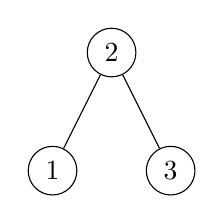
\begin{tikzpicture}[nodes={draw, circle}, -]
    \node{2}
    child { node {1} }
    child { node {3} };
    \end{tikzpicture}
    \caption{An undirected labelled graph with 3 nodes, $\mathcal{V}=\left\lbrace1,2,3\right\rbrace$ and $\mathcal{E}=\left\lbrace\left\lbrace1,2\right\rbrace\left\lbrace2,3\right\rbrace\right\rbrace$.}
    \label{fig:und_graph}
\end{figure} $\newline$
The \textit{neighbours} of node $i$ are defined as all nodes in $\mathcal{G}$ with an edge to node $i$,
\begin{equation*}
    \hbox{ne}\left(i\right)=\left\lbrace j\in\mathcal{V}:\left\lbrace i,j\right\rbrace\in\mathcal{E}\right\rbrace.
\end{equation*}
This definition can be extended to a set $A\subset\mathcal{V}$, where the neighbours of $A$ are defined as
\begin{equation*}
    \hbox{ne}\left(A\right)=\bigcup_{i\in A}\hbox{ne}\left(i\right)\setminus A.
\end{equation*}
A \textit{path} from $i_1$ to $i_m$ is defined as a sequence of certain nodes in $\mathcal{V}, i_1,i_2,...,i_m$, for which $\left(i_j,i_{j+1}\right)\in\mathcal{E}$ for $j=1,...,m-1$. Two nodes $i\notin C$ and $j\notin C$ are \textit{separated} by a subset $C\subset\mathcal{V}$, if every path from $i$ to $j$ contains at least one node from $C$. Two disjoint sets $A\subset\mathcal{V}\notin C$ and $B\subset\mathcal{V}\notin C$ are separated by $C$, if all $i\in A$ and $j\in B$ are separated by $C$, that is, it is not possible to "wander" on the graph from somewhere in $A$ and end somewhere in $B$ without crossing $C$.\\
If $i$ and $j$ are neighbours in $\mathcal{G}$, this can be expressed by $i\overset{\mathcal{G}}{\sim}j$ or $i\sim j$ for the case where the graph is implicit. It follows that $i\sim j\Longleftrightarrow j\sim i$. \\
Let $A$ be a subset of $\mathcal{V}$. A \textit{subgraph} $\mathcal{G}^A$ is a graph restricted to $A$, i.e., the graph obtained after removing all nodes that do not belong to $A$ and all edges where at least one node does not belong to $A$. $\mathcal{G}^A=\left\lbrace\mathcal{V}^A,\mathcal{E}^A\right\rbrace$, where $\mathcal{V}^A=A$ and 
\begin{equation*}
    \mathcal{E}^A = \left\lbrace\left\lbrace i,j\right\rbrace\in\mathcal{A} \hbox{ and } \left\lbrace i,j\right\rbrace\in A\times A\right\rbrace.
\end{equation*}
Let $\mathcal{G}$ be the graph in \autoref{fig:und_graph} and $\mathcal{A}=\left\lbrace2,3\right\rbrace$, then $\mathcal{V}^A=\left\lbrace2,3\right\rbrace$ and $\mathcal{E}^A=\left\lbrace\left\lbrace 1,2\right\rbrace\right\rbrace$\autocite[Cf.][]{rue2005gaussian}.
\subsection{The Exponential Family}
In statistics and probability theory, the \textit{exponential family} is a parametric set of probability distributions of a specific form. The distribution of a random variable $\pmb{y}$ belongs to the exponential family if the discrete or continuous density with respect to a $\sigma$-finite measure of $\pmb{y}$ has the form
\begin{equation}
    f(\pmb{y}|\pmb{\theta}, \lambda)=\exp\left(\frac{\pmb{y}^T\pmb{\theta} - b(\pmb{\theta})}{\lambda}+c(\pmb{y},\lambda) \right),
\end{equation}
with $c(\pmb{y},\lambda)\geq 0$ and measurable. $\pmb{\theta}\in\Theta\subset\mathbb{R}^q$ is the \textit{natural} or \textit{canonical} parameter of the exponential family, while $\lambda > 0$ is a \textit{dispersion} or \textit{nuisance} parameter. The natural parameter space $\Theta$ is the set of all $\pmb{\theta}$ satisfying $0<\int\exp\left(\left(\pmb{y}^T\pmb{\theta} - b(\pmb{\theta})\right)/\lambda+c(\pmb{y},\lambda) \right)d\pmb{y}< \infty$. Moreover, $b(\pmb{\theta})$ is a twice differentiable  function and all moments of $\pmb{y}$ exist. Specifically, 
\begin{alignat}{3}
    \mathbb{E}_{\pmb{\theta}}(\pmb{y}) &= \mu(\pmb{\theta}) =& \frac{\partial b(\pmb{\theta})}{\partial\pmb{\theta}} \\
    \hbox{Cov}_{\pmb{\theta}}(\pmb{y}) &= \pmb{\Sigma}(\pmb{\theta}) =& \lambda\frac{\partial^2b(\pmb{\theta})}{\partial\pmb{\theta}\partial\pmb{\theta}^T}.
\end{alignat}
The covariance matrix $\pmb{\Sigma}(\pmb{\theta})$ is positive definite in $\Theta^0$, therefore $\mu:\Theta^0\rightarrow  M = \mu\left(\Theta^0\right)$ is injective. By substituting the inverse function $\theta(\mu)$ into $\frac{\partial^2b(\pmb{\theta})}{\partial\pmb{\theta}\partial\pmb{\theta}^T}$, the variance function 
\begin{equation}
    v(\mu)=\frac{\partial^2b(\pmb{\theta}(\mu))}{\partial\pmb{\theta}\partial\pmb{\theta}^T}
\end{equation}
is given and the covariance can be written as
\begin{equation}
    \hbox{Cov}_{\pmb{\theta}}(\pmb{y}) = \lambda v(\mu).
\end{equation}
Important members of the exponential family are the normal, binomial, Poisson, gamma and multivariate normal distribution\autocite[Cf.][]{fahrmeir2013multivariate}.
\subsection{The Multivariate Normal Distribution}
The density of a normally distributed random variable $\pmb{x}=\left(x_1,...,x_n\right)^T, n<\infty$ with mean vector $\pmb{\mu}$ ($n\times1$) and SPD covariance matrix $\Sigma$ ($n\times n$) is
\begin{equation}
    \pi\left(\pmb{x}\right)=\left(2\pi\right)^{-n/2}|\pmb{\Sigma}|^{-1/2}\exp\left(-\frac{1}{2}\left(\pmb{x}-\pmb{\mu}\right)^T\pmb{\Sigma}^{-1}\left(\pmb{x}-\pmb{\mu}\right)\right),\hspace{5pt}\pmb{x}\in\mathbb{R}^n
\end{equation}
Here, $\mu_i=\mathbb{E}\left[x_i\right]$, $ \Sigma_{ij}=\hbox{Cov}\left(x_i,x_j\right)$, $ \Sigma_{ii}=\hbox{Var}\left(x_i\right) > 0$ and $\hbox{Corr}\left(x_i,x_j\right)=\Sigma_{ij}/\left(\Sigma_{ii}\Sigma_{jj}\right)^{1/2}$. This is written as $\pmb{x}\sim\mathcal{N}\left(\pmb{\mu},\pmb{\Sigma}\right)$. For $n=1$, $\mu=0$ and $\Sigma_{11}=1$ the standard normal distribution is obtained. \\
$\pmb{x}$ is now split up into $\pmb{x}=\left(\pmb{x}_{\pmb{A}}^T,\pmb{x}_{\pmb{B}}^T\right)$ and $\pmb{\mu}$ and $\pmb{\Sigma}$ are divided accordingly:
\begin{equation*}
    \pmb{\mu} = \begin{pmatrix}\pmb{\mu}_{\pmb{A}} \\ \pmb{\mu}_{\pmb{B}}\end{pmatrix} \hspace{10pt}\hbox{ and }\hspace{10pt} \pmb{\Sigma}=\begin{pmatrix}\pmb{\Sigma}_{\pmb{AA}} & \pmb{\Sigma}_{\pmb{AB}}\\\pmb{\Sigma}_{\pmb{BA}} & \pmb{\Sigma}_{\pmb{BB}}\end{pmatrix}.
\end{equation*}
Some basic properties of the multivariate normal distribution are the following.
\begin{itemize}
    \item[1.] $\pmb{x}_{\pmb{A}}\sim\mathcal{N}\left(\pmb{\mu}_{\pmb{A}}, \pmb{\Sigma}_{\pmb{AA}}\right)$.
    \item[2.] $\pmb{\Sigma}_{\pmb{AB}}=\pmb{0}$ precisely when $\pmb{x}_{\pmb{A}}$ and $\pmb{x}_{\pmb{B}}$ are independent.
    \item[3.] The conditional distribution $\pi\left(\pmb{x}_{\pmb{A}}|\pmb{x}_{\pmb{B}}\right)$ is $\mathcal{N}\left(\pmb{\mu}_{\pmb{A}|\pmb{B}}, \pmb{\Sigma}_{\pmb{A}|\pmb{B}}\right)$, where
    \begin{align*}
        \pmb{\mu}_{\pmb{A}|\pmb{B}} &= \pmb{\mu}_{\pmb{A}}+\pmb{\Sigma}_{\pmb{AB}}+\pmb{\Sigma}_{\pmb{BB}}^{-1}\left(\pmb{x}_{\pmb{B}}-\pmb{\mu}_{\pmb{B}}\right) \hbox{ and} \\
        \pmb{\Sigma}_{\pmb{A}|\pmb{B}} &= \pmb{\Sigma}_{\pmb{AA}}-\pmb{\Sigma}_{\pmb{AB}}\pmb{\Sigma}_{\pmb{BB}}^{-1}\pmb{\Sigma}_{\pmb{BA}}.
    \end{align*}
    \item[4.] If $\pmb{x}\sim\mathcal{N}\left(\pmb{\mu}, \pmb{\Sigma}\right)$ and $\pmb{x}'\sim\mathcal{N}\left(\pmb{\mu'}, \pmb{\Sigma'}\right)$ are independent, then $\pmb{x}+\pmb{x'}\sim\mathcal{N}\left(\pmb{\mu}+ \pmb{\mu'}, \pmb{\Sigma}+ \pmb{\Sigma'}\right)$\autocite[Cf.][]{rue2005gaussian}.
\end{itemize}
\section{Conjugate Priors}
One property of exponential families is that they have conjugate priors, which is an important property in Bayesian statistics. If the posterior distribution $p\left(\pmb{\theta}|\pmb{x}\right)$ and the prior distribution $p\left(\pmb{\theta}\right)$ belong to the same probability distribution family, the prior and posterior distributions are called \textit{conjugate} distributions. Furthermore, the prior for the likelihood function $p\left(\pmb{x}|\pmb{\theta}\right)$ is called the \textit{conjugate prior}. The term was introduced by Raiffa and Schlaifer\autocite[Cf.][]{raiffaapplied}, and the property that all members of the exponential family have conjugate priorities was shown by Diaconis and Ylvisaker\autocite[Cf.][]{diaconis1979conjugate}.
\subsection{Penalised Complexity Priors}
One issue when selecting the prior distribution of a particular parameter is that it is not always intuitive when it comes to understanding and interpreting this distribution, something that is essential to ensure that it behaves as intended by the user. This problem can be addressed by using \textit{penalised complexity priors}, which is a methodology that penalises the complexity of model components in relation to deviation from simple base model formulations.\\
PC priors provide a systematic and unified approach to calculating priority distributions for parameters of model components by using an inherited nested structure. This structure contains two models, the base model and a flexible version of the model. The first of the two is generally characterised by a fixed value of the relevant parameter, while the second version is considered a function of the random parameter. By penalising the deviation from the flexible model to the fixed base model, the PC prior is calculated.
\subsubsection{The Principles Behind PC Priors}
Four main principles should be followed to calculate priorities in a consistent way and to understand their properties.
\subsubsection*{Support to Occam's Razor} 
Let $\pi\left(x|\xi\right)$ denote the density of a model component $x$ and $\xi$ the parameter to which a prior distribution is to be assigned. The base model is characterised by a density $\pi\left(x|\xi=\xi_0\right)$, where $\xi_0$ is a fixed value. The prior for $\xi$ should be such that proper shrinkage is given to $\xi_0$. The simplicity of the model is therefore prioritised over the complexity of the model, preventing overfitting.
\subsubsection*{Penalisation of Model Complexity} 
Let $f_1=\pi\left(x|\xi\right)$ and $f_0\left(x|\xi=\xi_0\right)$ denote the flexible model and the base model respectively. The complexity of $f_1$ compared to $f_0$ is characterised using the Kullback-Leibler divergence to calculate a measure of complexity between the two models,
\begin{equation}
    \hbox{KLD}\left(f_1||f_2\right) = \int f_1\left(x\right)\log\left(\frac{f_1\left(x\right)}{f_0\left(x\right)}\right)dx.
\end{equation}
This can be used to measure the information that is lost when $f_1$ is approximated by the simpler model $f_0$. For multinormal densities with zero mean, the calculation simplifies to
\begin{equation}
    \hbox{KLD}\left(f_1||f_0\right) = \frac{1}{2}\left(\hbox{trace}\left(\pmb{\Sigma}_0^{-1}\pmb{\Sigma}_1\right)-n-\ln\left(\frac{\left|\pmb{\Sigma}_1\right|}{\left|\pmb{\Sigma}_0\right|}\right)\right),
\end{equation}
where $f_i\sim\mathcal{N}\left(0,\pmb{\Sigma}_i\right), i=0,1$, while $n$ represents the dimension. For easier interpretation, the Kullback-Leibler divergence is transformed into a unidirectional distance measure
\begin{equation}
    d\left(\xi\right) = d\left(f_1||f_0\right)=\sqrt{2\hbox{KLD}\left(f_1||f_0\right)}
\end{equation}
which can be interpreted as a measure of distance from $f_1$ to $f_0$.
\subsubsection*{Constant Rate Penalisation}
The derivation of the PC prior is based on a system of constant rate penalisation, given by
\begin{equation}
    \frac{\pi_d\left(d\left(\xi\right)+\delta\right)}{\pi_d\left(d\left(\xi\right)\right)}=r^{\delta}, \hspace{20pt} d\left(\xi\right),\delta\geq0.
\end{equation}
$r\in\left(0,1\right)$ represents the constant decay rate and thus implies that the relative change in the priority distribution for $d\left(\xi\right)$ is independent of the actual distance. Therefore, $d\left(\xi\right)$ is exponentially distributed with density $\pi\left(d\left(\xi\right)\right)=\lambda\exp\left(-\lambda d\left(\xi\right)\right)$ and rate $\lambda = -\ln\left(r\right)$. By a standard variable change transformation, the corresponding PC prior for $\xi$ is given.
\subsubsection*{User-Defined Scaling}
Since $\lambda$ characterises the shrinkage properties of the prior, it is important that the rate can be chosen in an intuitive and interpretable way. One possibility is to determine $\lambda$ by including a probability statement of tail events, for example
\begin{equation}
    \mathbb{P}\left(Q\left(\xi\right) > U\right)=\alpha,
\end{equation}
where $U$ represents an assumed upper bound for an interpretable transformation $Q\left(\xi\right)$ and $\alpha$ denotes a small probability.
\subsubsection{PC Priors for AR(1)}
The first-order AR process is given by
\begin{equation}
    x_t=\phi x_{t-1}+\epsilon_t, \hspace{20pt}\epsilon\sim\mathcal{N}\left(0, \kappa^{-1}\right), \hspace{5pt} t=2,...,n,
\end{equation}
where $x_1$ is assumed to follow a normal distribution with mean $0$ and marginal precision $\tau=\kappa\left(1-\phi^2\right)$. The variables $\left\lbrace\epsilon_t\right\rbrace_{t=1}^n$ are independent and follow a $\mathcal{N}\left(0, \kappa\right)$ distribution. The AR(1) model represents an important special case of AR processes where the autocorrelation coefficient $\phi$ specifies the complete dependence structure.
\subsubsection*{Base Model: No Dependency in Time} 
The correlation matrix of an AR(1) is generally defined as $\pmb{\Sigma}_1=\left(\phi^{\left|i-j\right]}\right)$. In the case of no autocorrelation, white noise results and the correlation matrix is equal to the identity matrix, $\pmb{\Sigma}_0=\pmb{I}$. The distance function is defined as $d\left(\phi\right)=\sqrt{\left(1-n\right)\log\left(1-\phi^2\right)}$. According to the constant rate penalty principle, $d\left(\phi\right)$ is assigned an exponential prior with rate $\theta/\sqrt{n-1}$. This leads to a prior distribution that is invariant to $n$, and the PC for the one-lag autocorrelation is given by
\begin{equation}
    \pi\left(\phi\right)=\frac{\theta}{2}\exp\left(-\theta\sqrt{-\ln\left(1-\phi^2\right)}\right)\frac{|\phi|}{\left(1-\phi^2\right)\sqrt{-\ln\left(1-\phi^2\right)}}, \hspace{20pt} |\phi|<1,\theta>0.
\end{equation}
The rate parameter $\theta$ influences at what rate the prior shrinks towards the white noise base model. To infer $\theta$, a tail event is used. In the case of $\phi = 0$ a tail event can be defined by the fact that large absolute correlations are less likely, i.e..,
\begin{equation*}
    \mathbb{P}\left(|\phi|>U\right) = \alpha.
\end{equation*}
This implies that $\theta=-\ln\left(\alpha\right)/\sqrt{-\ln\left(1-U^2\right)}$
\subsubsection*{Base Model: No Change in Time} 
As an alternative to the base model for the AR(1) process, it can be assumed that the process remains constant in time ($\phi = 1$), thus representing a limiting random walk case, which is a non-stationary and singular process. To derive the PC prior for $\phi$, let $\pmb{\Sigma}_1=\left(\phi^{|i-j|}\right)$ and $\pmb{\Sigma}_0=\left(\phi_0^{|i-j|}\right)$, where $\phi_0$ is close to $1$ and $\phi<\phi_0$. The Kullback-Leibler divergence is
\begin{align*}
    &\hbox{KLD}\left(f_1\left(\phi\right)||f_0\right)=\\
    &\frac{1}{2}\left(\frac{1}{1-\phi_0^2}\left(n-2\left(n-1\right)\phi_0\phi+\left(n-2\right)\phi_0^2\right)-n-\left(n-1\right)\ln\left(\frac{1-\phi^2}{1-\phi_0^2}\right)\right).
\end{align*}
Considering the limit as $\phi_0\rightarrow1$, the distance is
\begin{align*}
    d\left(\phi\right)&=\underset{\phi_0\rightarrow1}{\lim}\sqrt{2\hbox{KLD}\left(f_1\left(\phi\right)||f_0\right)} \\
    &=\underset{\phi_0\rightarrow1}{\lim}\sqrt{\frac{2\left(n-1\right)\left(1-\phi\right)}{1-\phi_0^2}} = c\sqrt{1-\phi}, \hspace{20pt}|\phi|<1,
\end{align*}
constant for $c$, independent of $\phi$. Since $0\leq d\left(\phi\right)\leq c\sqrt{2}$, $d\left(\phi\right)$ is assigned a truncated exponential distribution with rate $\theta/c$, resulting in the following PC prior,
\begin{equation}
    \pi\left(\phi\right)=\frac{\theta\exp\left(-\theta\sqrt{1-\phi}\right)}{\left(1-\exp\left(-\sqrt{2}\theta\right)\right)2\sqrt{1-\phi}}, \hspace{20pt}|\phi|<1.
\end{equation}
To scale the prior in terms of $\theta$, $\left(U,\alpha\right)$ is determined in terms of $\mathbb{P}\left(\phi>U\right)=\alpha$. This equation is solved by
\begin{equation*}
    \frac{1-\exp\left(-\theta\sqrt{1-U}\right)}{1-\exp\left(-\sqrt{2}\theta\right)}=\alpha,
\end{equation*}
provided that $\alpha$ is larger than the lower limit $\sqrt{\left(1-U\right)/2}$\autocite[Cf.][]{sorbye2017penalised}.
\clearpage
\section{Markov-Chain-Monte-Carlo-Methods}
Markov chain Monte Carlo methods, also referred to as MCMC methods, are a set of algorithms that enable sampling from probability distributions based on the construction of Markov chains. After a sufficient number of iterations, the stationary distribution of a Markov chain can be taken as the desired distribution, with the quality of this distribution improving as the number of iterations increases. Most of the time, the construction of such a chain is relatively simple; the real challenge is to determine how many steps are needed before convergence towards the stationary distribution is achieved. MCMC methods are mostly used to compute numerical approximations of multidimensional integrals, for instance in Bayesian statistics or computational biology. The two main concepts used in MCMC methods are Monte Carlo integration and the aforementioned Markov chains, hence the name Markov Chain Monte Carlo.
\subsection{Monte Carlo Integration}
\textit{Monte Carlo integration} is a technique that uses the generation of random numbers for numerical computation of definite integrals and is especially useful for higher-dimensional integrals. The problem the method addresses is the computation of the integral
\begin{equation}
    \mathbb{E}_f\left[h\left(X\right)\right]=\int_\chi h(x)f(x)dx.
\end{equation}
The integral can be approximated by using a sample $\left(X_1,...,X_m\right)$ generated from $f$ and calculating the arithmetic mean
\begin{equation}
    \overline{h}_m=\frac{1}{m}\sum_{j=1}^mh\left(x_j\right).
\end{equation}
According to the Strong Law of Large Numbers, $\overline{h}_m$ is likely to converge to $\mathbb{E}_f\left[h\left(X\right)\right]$. When the expectation of $h^2$ under $f$ is finite, the convergence speed of $\overline{h}_m$ can be assessed. The variance too can be estimated from the sample $\left(X_1,...,X_N\right)$ through
\begin{equation}
    v_m=\frac{1}{m^2}\sum_{j=1}^m\left[h\left(x_j\right)-\overline{h}_m\right]^2.
\end{equation}
For $m$ large,
\begin{equation}
    \frac{\overline{h}_m-\mathbb{E}_f\left[h\left(X\right)\right]}{\sqrt{v_m}}
\end{equation}
is approximately distributed as a $\mathcal{N}(0,1)$ variable. This can be used for constructing a convergence test and to calculate confidence bounds for the approximation of $\mathbb{E}_f\left[h\left(X\right)\right]$\autocite[Cf.][]{robert2013monte}.
\subsection{Markov Chains}
Markov chains are stochastic processes that aim to provide the probability of the occurrence of future events. A Markov chain is defined by the fact that even if only a limited history is known, predictions about future developments can be made just as reliably as if the entire history of a process were known. Thus, the probability of moving from the current state to any state depends only on the current state of the chain. These probabilities are defined by a \textit{transition kernel}, which is a function $K$ on $\mathcal{X} \times \mathcal{B}\left(\mathcal{X}\right)$, such that
\begin{itemize}
    \item[i.] $\forall x\in\mathcal{X}, K\left(x, \cdot\right)$ is a probability measure;
    \item[ii.] $\forall A\in \mathcal{B}\left(\mathcal{X}\right), K\left(\cdot, A\right)$ is measureable.
\end{itemize}
In the discrete case, the transition kernel is a matrix $\pmb{K}$ with elements
\begin{equation*}
    \mathbb{P}_{xy}=\mathbb{P}\left(X_n=y|X_{n-1}=x\right), \hspace{20pt}x,y\in\mathcal{X}.
\end{equation*}
If $\mathcal{X}$ is continuous, the kernel denotes the conditional density $K\left(x,x^T\right)$ of the transition $K\left(x,\cdot\right)$,
\begin{equation*}
    \mathbb{P}\left(X\in A|x\right)=\int_AK\left(x,x^T\right)dx^T.
\end{equation*}
Given a transition kernel $K$, a sequence $X_0,X_1,...,X_n$ of random variables is a \textit{Markov chain} $\left(X_n\right)$, if, for any $t$, the conditional distribution of $X_t$ given the previous states is the same as the distribution of $X_t$ given the last state, $x_{t-1}$,
\begin{align}
    \mathbb{P}\left(X_{k+1}\in A|x_0,x_1,x_2,...,x_k\right) &= \mathbb{P}\left(X_{k+1}\in A|x_k\right) \nonumber\\
    &= \int_A K\left(x_k, dx\right). 
\end{align}
Markov chains can have certain properties that affect their long-term behaviour and are of particular importance for MCMC algorithms. Next, some of them will be introduced.
\subsubsection{Irreducibility} 
Irreducibility is critical to the construction of Markov chain Monte Carlo algorithms, as it ensures the convergence of such an algorithm. A Markov chain is \textit{irreducible} if all states communicate, that is, for all states $i$ and $j$ the probability of getting from $i$ to $j$ in finite time is true positive. \\
Formally speaking, given a measure $\varphi$, a Markov chain $\left(X_n\right)$ with transition kernel $K\left(x,y\right)$ is $\varphi$-\textit{irreducible}, if, for every $A\in B\left(\mathcal{X}\right)$ with $\varphi\left(A\right)>0$, there exists $n$ such that $K^n\left(x,A\right) \forall x\in\mathcal{X}$. The chain is \textit{strongly} $\varphi$-\textit{irreducible} if $n=1\forall$ measurable $A$.
\subsubsection{Periodicity} 
The behaviour of a Markov chain can sometimes be limited by deterministic constraints on the transitions from $X_n$ to $X_{n+1}$. For discrete chains, the \textit{period} of a state $w\in\mathcal{X}$ is defined as. 
\begin{equation*}
    d\left(w\right)=\hbox{g.c.d. } \lbrace m\geq 1;K^m\left(w,w\right)>0\rbrace,
\end{equation*}
with g.c.d the greatest common denominator. If a Markov chain is irreducible, the transition matrix can be written as a block matrix
\begin{equation}
    \pmb{P}=\begin{pmatrix}
    0 & \pmb{D}_1 & 0 & \dots & 0\\
    0 & 0 & \pmb{D}_2 & \dots & 0 \\
    \vdots & \vdots & \ddots  \\
    \pmb{D}_d & 0 & 0 & & 0
    \end{pmatrix},
\end{equation}
It is evident that at every $d$-th step there is a return to the initial group. There exists only one value for the period when a chain is irreducible. If this value is 1, the irreducible chain is \textit{aperiodic}.
 \subsubsection{Transience and Recurrence} 
To guarantee an acceptable approximation of a simulated model, a Markov chain needs to have good stability properties. Irreducibility is not strong enough to ensure that the trajectory of $\left(X_n\right)$ enters $A$ often enough. This leads to the formalisation of \textit{recurrence} and \textit{transience}.  \\
In a finite space $\mathcal{X}$, a state $w\in\mathcal{X}$ is \textit{transient} if it is finitely often visited and \textit{recurrent} if it is almost certainly infinitely often visited. \\
For irreducible chains, these two properties are properties of the chain, not of a particular state. 
\subsubsection{Ergodicity}
When looking at a Markov Chain $\left(X_n\right)$ from a temporal point of view, it is essential to establish to what the chain is converging. A natural candidate for the limiting distribution is the stationary distribution $\pi$ which leads to the need to define sufficient conditions on $\left(X_n\right)$ for $X_n$ to be asymptotically distributed according to $\pi$. There are several conditions that can be imposed on the convergence of $P^n$, the distribution of $X_n$ to $\pi$. The most fundamental ans important is that of \textit{ergodicity}, that is, independence of initial conditions. \\
If a Markov chain $\left(X_n\right)$ is both aperiodic and positive recurrent, it is called an \textit{ergodic} Markov chain.
\subsubsection{Stationary distribution} 
A chain $\left(X_n\right)$ is more stable if the marginal distribution of $X_n$ is independent of $n$. This is a requirement for the existence of a probability distribution $\pi$ such that $X_{n+1}\sim\pi$ if $X_n\sim\pi$. Markov chain Monte Carlo methods rely on the fact that this condition can be satisfied. \\
A $\sigma$-finite measure $\pi$ is \textit{invariant} for the transition kernel $K\left(\cdot,\cdot\right)$ if \begin{equation*}
    \pi\left(B\right)=\int_\mathcal{X}K\left(x,B\right)\pi(dx), \hspace{20pt} \forall B\in\mathcal{B}\left(\mathcal{X}\right).
\end{equation*}
This distribution is referred to as \textit{stationary} if $\pi$ is a probability measure, as $X_0\sim\pi$ implies that $X_n\sim\pi$ is $\forall n$. An irreducible Markov chain has a stationary distribution precisely if it is positively recurrent. The distribution is then given by
\begin{equation}
    \pi_x=\left(\mathbb{E}_x\left[\tau_x\right]\right)^{-1}, \hspace{20pt} x\in\mathcal{X},
\end{equation}
where $\mathbb{E}_x\left[\tau_x\right]$ can be interpreted as the average number of transitions between two passages in $x$. \\
In practice, the stationary distributions are often of special interest. If these distributions are defined as the starting distribution of $X_0$, then all following distributions of the states $X_n$ for any $n$ are equal to the starting distribution. The interesting question here is when such distributions exist and when any distribution converges against a stationary distribution of this kind\autocite[Cf.][]{robert2013monte}.
\subsection{The Metropolis-Hastings Algorithm}
Having established the basics of MCMC methods, one of the best known MCMC algorithms, the Metropolis-Hastings algorithm, is introduced next. It is a procedure for drawing random samples from a probability distribution from which direct sampling is difficult if a function proportional to the \textit{target density} $f$ is known. This function $q\left(\pmb{y}|\pmb{x}\right)$ is called the \textit{proposal density} and must be easy to simulate in order for the Metropolis-Hastings algorithm to be implementable. Moreover, it must be either explicitly present or \textit{symmetric}, meaning $q\left(\pmb{x}|\pmb{y}\right)=q\left(\pmb{y}|\pmb{x}\right)$. \\
The Metropolis-Hastings algorithm of a target density $f$ and proposal density $q$ produces a Markov chain $\left(X^{(t)}\right)$ by the following transition.
\begin{algorithm}[H]
\caption{The Metropolis-Hastings Algorithm}
\begin{algorithmic}[1]
\Statex Given $f\left(\pmb{x}\right)$ and $q\left(\pmb{y}|\pmb{x}\right)$
\State Initialisation: Choose arbitrary $x_t$ as the first sample
\For{each iteration $t$}
    \State Generate $Y_t\sim q\left(\pmb{y}|x^{(t)}\right)$
    \State Take 
    \begin{align}
        X^{(t+1)}&=\begin{cases}
        Y_t & \hbox{with probability } \mathbb{P}\left(x^{(t)}, Y_t\right) \\
        x^{(t)} & \hbox{with probability } 1-\mathbb{P}\left(x^{(t)}, Y_t\right)
        \end{cases} \nonumber \\
    \hbox{where} \nonumber\\
    \mathbb{P}\left(x,y\right) &= \min\left\lbrace\frac{f\left(\pmb{y}\right)}{f\left(\pmb{x}\right)}\frac{q\left(\pmb{x}|\pmb{y}\right)}{q\left(\pmb{y}|\pmb{x}\right)}, 1\right\rbrace.
    \end{align} 
    \EndFor
\end{algorithmic}
\end{algorithm}  $\newline$
$\mathbb{P}\left(x,y\right)$ is the \textit{Metropolis-Hastings acceptance probability}. \\
The algorithm always accepts values $y_t$ that lead to an increase in the ratio $f\left(y_t\right)/q\left(y_t|x^{(t)}\right)$ compared to the previous value $f\left(x^{(t)}\right)/q\left(x^{(t)}|y_t\right)$. In the symmetric case, the acceptance probability simplifies to
\begin{equation*}
     \mathbb{P}\left(x,y\right) = \min\left\lbrace\frac{f\left(\pmb{y}\right)}{f\left(\pmb{x}\right)}, 1\right\rbrace.
\end{equation*}
If the Markov chain starts with a value $x^{(0)} > 0$, then $f\left(x^{(t)}\right) > 0 \forall t\in\mathbb{N}$ since the values of $y$ such that $f\left(y_t\right) = 0$ will all be rejected by the algorithm. As the number of iterations $t$ increases, the distribution of saved states $x_0,...,x_t$ will converge towards the target density $f(\pmb{x})$\autocite[Cf.][]{robert2013monte}.
% hier könnten noch Diagnostics für MCMC methods / MH Algorithm sein, z.b. Traceplot. Außerdem sample mean für schätzung des posterior mean und sample variance für schätzung der varianz
\subsection{The Gibbs Sampler}
Gibbs-Sampling is a special case of the Metropolis-Hastings Algorithm, that is used to generate a sequence of samples of the joint probability distribution of two or more random variables. The aim of the method is to approximate this unknown joint probability distribution. Gibbs sampling is especially suitable when the joint distribution of a random vector is unknown, but the conditional distribution of each random variable is known. The underlying principle is to repeatedly select a variable and generate a value according to its conditional distribution, depending on the values of the other variables. During this iteration step, the values of the other variables remain unchanged. A Markov chain can be derived from the resulting sequence of sample vectors, and it can be shown that the stationary distribution of this Markov chain is precisely the sought joint distribution of the random vector.
\subsubsection{The Two-Stage Gibbs Sampler}
A general introduction to Gibbs sampling is the two-stage Gibbs sampler, which is applicable to a wide range of statistical models that do not demand the generality of the multi-stage Gibbs sampler. \\
Implementing the algorithm is straightforward. If the random variables $X$ and $Y$ have a joint density $f\left(\pmb{x},\pmb{y}\right)$, the two-stage Gibbs sampler generates a Markov chain $\left(X_t,Y_t\right)$ as shown below.
\begin{algorithm}
\caption{The Two-Stage Gibbs Sampler}
\begin{algorithmic}[1]
\Statex Take $X_0=x_0$
\For{each iteration $t$}
    \State Generate $Y_t\sim f_{Y|X}\left(\cdot|x_{t-1}\right)$
    \State Generate $X_t\sim f_{X|Y}\left(\cdot|y_t\right)$
    \EndFor
\end{algorithmic}
\end{algorithm} 
$f_{Y|X}$ and $f_{X|Y}$ represent the conditional densities associated with $f$. It is worth noting that not only $\left(X_t,Y_t\right)$ is a Markov chain, but also the subsequences $\left(X_t\right)$ and $\left(Y_t\right)$ are. 
\subsubsection*{Normal Bivariate Gibbs Sampler} 
In the case of the bivariate normal density
\begin{equation*}
    \left(X,Y\right)\sim \mathcal{N}_2\left(0,  \begin{pmatrix}
    1 & p \\ p & 1
    \end{pmatrix}\right)
\end{equation*}
the Gibbs sampler reads as follows.
\begin{algorithm}
\caption{The Two-Stage Gibbs Sampler for a normal distribution}
\begin{algorithmic}[1]
\Statex Given $y_t$
\For{each iteration $t$}
    \State Generate $X_{t+1}|y_t \sim \mathcal{N}\left(py_t, 1-p^2\right)$
    \State Generate $Y_{t+1}|x_{t+1}\sim\mathcal{N}\left(px_{t+1},1-p^2\right)$
    \EndFor
\end{algorithmic}
\end{algorithm} 
\subsubsection{The Multi-Stage Gibbs Sampler}
Let $p>1$, then the random variable $X\in\mathcal{X}$ can be written as $X=\left(X_1,...,X_p\right)$, where the $X_i$'s are either one-dimensional or multidimensional. Moreover, assume that a simulation is possible from the corresponding univariate conditional densities $f_1,...,f_p$, i.e., 
\begin{equation*}
    X_i|\pmb{x}_{-i}\sim f_i\left(x_i|\pmb{x}_{-i}\right)
\end{equation*}
can be simulated for $i=1,...,p$. The Gibbs sampler is then specified by the following transition from $X^{(t)}$ to $X^{(t+1)}$:
\begin{algorithm}[H]
\caption{The Multi-Stage Gibbs Sampler}
\begin{algorithmic}[1]
\Statex Given $x^{(t)}=\left(x_1^{(t)},...,x_p^{(t)}\right)$, generate
\State $X_1^{(t+1)}\sim f_1\left(x_1|x_2^{(t)},...,x_p^{(t)}\right)$;
\State $X_2^{(t+1)}\sim f_2\left(x_2|x_1^{(t)},x_3^{(t)},...,x_p^{(t)}\right)$;
\Statex $\vdots$
\Statex $X_p^{(p+1)}\sim f_p\left(x_p|\pmb{x}_{-p}\right)$
\end{algorithmic}
\end{algorithm} $\newline$
$f_1,...,f_p$ are referred to as the \textit{full conditionals} and these are the only densities used for simulation. Hence, all simulations can be univariate, even for a high-dimensional problems.
\clearpage
\section{Latent Gaussian Models and INLA}
In recent years, a growing amount of georeferenced data has become available, leading to an increased need for appropriate statistical modeling to handle large and complex datasets. Bayesian hierarchical models have proven to be effective in capturing complex stochastic structures in spatial processes. A large proportion of these models are based on latent Gaussian models, a subclass of structured additive regression models. 
\subsection*{Notation and Basic Properties}
\label{sec:notation}
For structured additive regression models, the distribution of the response variable $y_i$ is assumed to be a member of the exponential family, with the mean $\mu_i$ linked to a structured additive predictor $\eta_i$ by a link function $g\left(\cdot\right)$ such that $g\left(\mu_i\right)=\eta_i$. The predictor $\eta_i$  takes into account the effect of multiple covariates in an additive way,
\begin{equation}\label{eq:predictor}
    \eta_i=\alpha+\sum_{j=1}^{n_f}f^{(j)}\left(u_{ji}\right)+\sum_{k=1}^{n_{\beta}}\beta_kz_{ki}+\epsilon_i.
\end{equation}
The $\left\lbrace f^{(j)}\left(\cdot\right)\right\rbrace$s are unknown functions of the covariates $u$, while the $\left\lbrace\beta_k\right\rbrace$s represent the linear effect of the covariates $z$ and the $\epsilon_i$s are unstructured terms. Latent Gaussian models assign a Gaussian prior to $\alpha$, $\left\lbrace f^{(j)}\left(\cdot\right)\right\rbrace$ and $\left\lbrace\epsilon_i\right\rbrace$. In the following $\pmb{x}$ shall denote the vector of all latent Gaussian variables ($\left\lbrace\eta_i\right\rbrace$, $\alpha$, $\left\lbrace f^{(j)}\right\rbrace$ and $\left\lbrace\beta_k\right\rbrace$) and $\pmb{\theta}$ the vector of hyperparameters. \\
The conditional density $\pi\left(\pmb{x}|\theta_1\right)$ is Gaussian with an assumed zero mean and precision matrix $\pmb{Q}\left(\theta_1\right)$. The Gaussian density $\mathcal{N}\left(\mu,\pmb{\Sigma}\right)$ with mean $\mu$ and covariance $\pmb{\Sigma}$ at configuration $x$ is denoted by $\mathcal{N}\left(\pmb{x};\mu,\pmb{\Sigma}\right)$. For simplicity, $\left\lbrace\eta_i\right\rbrace$ has been included instead of $\left\lbrace\epsilon_i\right\rbrace$. \\
The distribution for the $n_d$ observational variables $y=\left\lbrace y_i:i\in\mathcal{I}\right\rbrace$ is denoted by $\pi\left(\pmb{y}|\pmb{x}, \theta_2\right)$ and is assumed conditionally independent given $\pmb{x}$ and $\theta_2$. Let $\pmb{\theta}=\left(\theta_1^T,\theta_2^T\right)^T$ with $\dim\left(\pmb{\theta}\right)=m$. For non-singular $\pmb{Q}\left(\pmb{\theta}\right)$ the posterior is given by
\begin{align}
    \pi\left(\pmb{x},\pmb{\theta}|\pmb{y}\right)&\propto\pi\left(\pmb{\theta}\right)\pi\left(\pmb{x}|\pmb{\theta}\right)\prod_{i\in I}\pi\left(y_i|x_i,\pmb{\theta}\right) \nonumber\\
    &\propto \pi\left(\pmb{\theta}\right)\left|\pmb{Q}\left(\pmb{\theta}\right)\right|^{1/2}\exp\left[-\frac{1}{2}\pmb{x}^TQ\left(\pmb{\theta}\right)\pmb{x}+\sum_{i\in I}\log\left\lbrace\pi\left(y_i|x_i,\pmb{\theta}\right)\right\rbrace\right].
\end{align}
Most latent Gaussian models satisfy two basic properties:
\begin{itemize}
    \item[1.] The latent field $\pmb{x}$ is of large dimension, $n\approx10^2-10^5$. Therefor, the latent field is a Gaussian Markov random field with sparse precision matrix $\pmb{Q}\left(\pmb{\theta}\right)$.
    \item[2.] The number of hyperparameters, $m$, is small, $m\leq6$.
\end{itemize}
In most cases, both properties are required to produce fast inference, and thus these will be assumed to be true for the remainder of this work\autocite[Cf.][]{rue2009approximate}.
\subsection{Applications for Latent Gaussian Models}
Latent Gaussian models can be employed in a vast range of different domains, in fact most structured Bayesian models are of this particular form. Some of these domains are presented below.
\subsubsection*{Regression Models}
Bayesian generalised linear models correspond to the linear relationship $\eta_i=\alpha+\sum_{k=1}^{n_\beta}\beta_k z_{ki}.$ Either the linear relationship of the covariates, random effects or both can be introduced using the $f\left(\cdot\right)$ terms. Smooth covariate effects are frequently modeled using penalised spline models or random walk models, continuous indexed spline models or Gaussian processes. The incorporation of random effects allows for the consideration of overdispersion caused by unobserved heterogeneity or correlation in longitudinal data and can be introduced by defining $f\left(u_i\right)=f_i$ and $\left\lbrace f_1\right\rbrace$ to be independent, zero mean and Gaussian.
\subsubsection*{Dynamic Models}
Temporal dependence can be introduced by using $i$ in \eqref{eq:predictor} as temporal index $t$ and defining $f\left(\cdot\right)$ and $\pmb{u}$ such that $f\left(u_t\right)=f_t$. Both a discrete-time and a continuous-time autoregressive model can be modeled by $\left\lbrace f_t\right\rbrace$. Furthermore, a seasonal effect or the latent process of a structured time series model can be modeled. Alternatively, a smooth temporal function in the same sense as for regression models can be represented by $\left\lbrace f_t\right\rbrace$.
\subsubsection*{Spatial and Spatio-Temporal Models}
Similar to the previous type of model, spatial dependence can be modeled by a spatial covariate $\pmb{u}$ such that $f\left(u_s\right)=f_s$, where $s$ denotes the spatial location or region $s$. The stochastic model for $f_s$ is constructed to promote spacial smooth realisations of some sort. Popular models of this type include the Besag-York-Mollié\autocite[Cf.][]{besag1991bayesian} model with extensions for regional data, continuous indexed Gaussian models and texture models. The dependence between spatial and temporal covariates can be achieved either by using a spatio-temporal covariate $(s,t)$ or a corresponding spatio-temporal Gaussian field.\\
Often the final model consists of a sum of several components, e.g. a spatial component, random effects and both linear and smooth effects of some covariates. In order to separate the effects of the different components in \eqref{eq:predictor}, sometimes linear or sum-to-zero constraints can be imposed\autocite[Cf.][]{rue2009approximate}.
\subsection{The MCMC Approach to Inference}
The usual approach to inference for latent Gaussian models involves the previously introduced Markov chain Monte Carlo methods. Due to several factors, these methods may perform poorly when applied to such models. One factor is the interdependence of the components of the latent field $\pmb{x}$ while another is that $\pmb{\theta}$ and $\pmb{x}$ are highly dependent on each other, especially for large $n$. The first of these problems can potentially be overcome by constructing a joint proposal based on a Gaussian approximation of the full conditional of $\pmb{x}$, while the second problem requires, at least in part, a joint update of $\pmb{\theta}$ and $\pmb{x}$. There are several proposals to solve these shortcomings, but MCMC sampling continues to show poor performance from the end user's point of view\autocite[Cf.][]{rue2009approximate}.
\subsection{Gaussian Random Fields}
Let $\pmb{s} = \left(s_1,...,s_n\right)^T$ be a vector of locations. A \textit{Gaussian random field} (GRF)
\begin{equation}
    \left\lbrace Z(s):s\in D\subset\mathbb{R}^2\right\rbrace
\end{equation}
is a set of random variables where the observations occur in a continuous domain and where each finite set of random variables follows a multivariate normal distribution. A random process $Z\left(\cdot\right)$ is strictly stationary if it is invariant to shifts, i.e., if for each set of locations and each $h\in\mathbb{R}^2$ the distribution of $\pmb{Z(s)}=\left(Z\left(s_1\right),... ,Z\left(s_n\right)\right)$ is equal to that of $\pmb{Z(s+h)}=\left(Z\left(s_1+h\right),...,Z\left(s_n+h\right)\right)$. A less constraining requirement is given by second-order stationarity. Under this condition, the process has a constant mean value
\begin{equation}
    \mathbb{E}\left[\pmb{Z(s)}\right] = \mu, \hspace{20pt}\forall s\in D,
\end{equation}
and the covariances depend only on the differences between locations
\begin{equation}
    \hbox{Cov}\left(\pmb{Z(s)}, \pmb{Z(s+h)}\right)=C\left(\pmb{h}\right), \hspace{20pt}\forall \pmb{s}\in D,\,\forall \pmb{h}\in\mathbb{R}^2.
\end{equation}
Furthermore, if the covariances depend only on the distances between the locations and not on the directions, the process is called isotropic. Else, the process is anisotropic. An intrinsically stationary process has a constant mean value and satisfies
\begin{equation}
    \hbox{Var}\left(Z\left(s_i\right)-Z\left(s_j\right)\right)=2\gamma\left(s_i-s_j\right),\hspace{20pt}\forall s_i,s_j.
\end{equation}
$2\gamma\left(\cdot\right)$ is the variogram and $\gamma\left(\cdot\right)$ is called the semivariogram. Under the assumption of intrinsic stationarity, the constant-mean assumption implies
\begin{equation*}
    2\gamma\left(\pmb{h}\right)=\hbox{Var}\left(\pmb{Z(s+h)}-\pmb{Z(s)}\right)=\mathbb{E}\left[\left(\pmb{Z(s+h)}-\pmb{Z(s)}\right)^2\right],
\end{equation*}
and the estimation of the semivariogram can be obtained using the empirical semivariogram as follows:
\begin{equation}
    2\widehat{\gamma}\left(\pmb{h}\right)=\frac{1}{\left|N\left(\pmb{h}\right)\right|}\sum_{N\left(\pmb{h}\right)}\left(Z\left(s_i\right)-Z\left(s_j\right)\right)^2,
\end{equation}
where $N\left(\pmb{h}\right)=\left\lbrace\left(s_1,s_j\right):s_i-s_j=\pmb{h}, i,j=1,...,n\right\rbrace$ denotes the number of pairs and $\left|N\left(\pmb{h}\right)\right|$ the number of distinct pairs. For isotropic processes, the semivariogram is a function of distance $h=\left|\left|\pmb{h}\right|\right|$.   \\
Plotting the empirical semivariogram against the separation distance conveys essential information regarding the continuity and spatial variability of the process. Given relatively short distances, the semivariogram tends to be small but increases with distance, indicating the similarity of observations in close proximity. The semivariogram levels off to a nearly constant value, also called the sill, as the separation distance increases, indicating a decrease in spatial dependence with distance within the range and no spatial correlation outside the range, which is reflected in a nearly constant variance. If there is a discontinuity or a vertical jump at the origin, the process has a nugget effect, which is often due to a measurement error, but may also be indicative of a spatially discontinuous process.
\begin{figure}
    \centering
    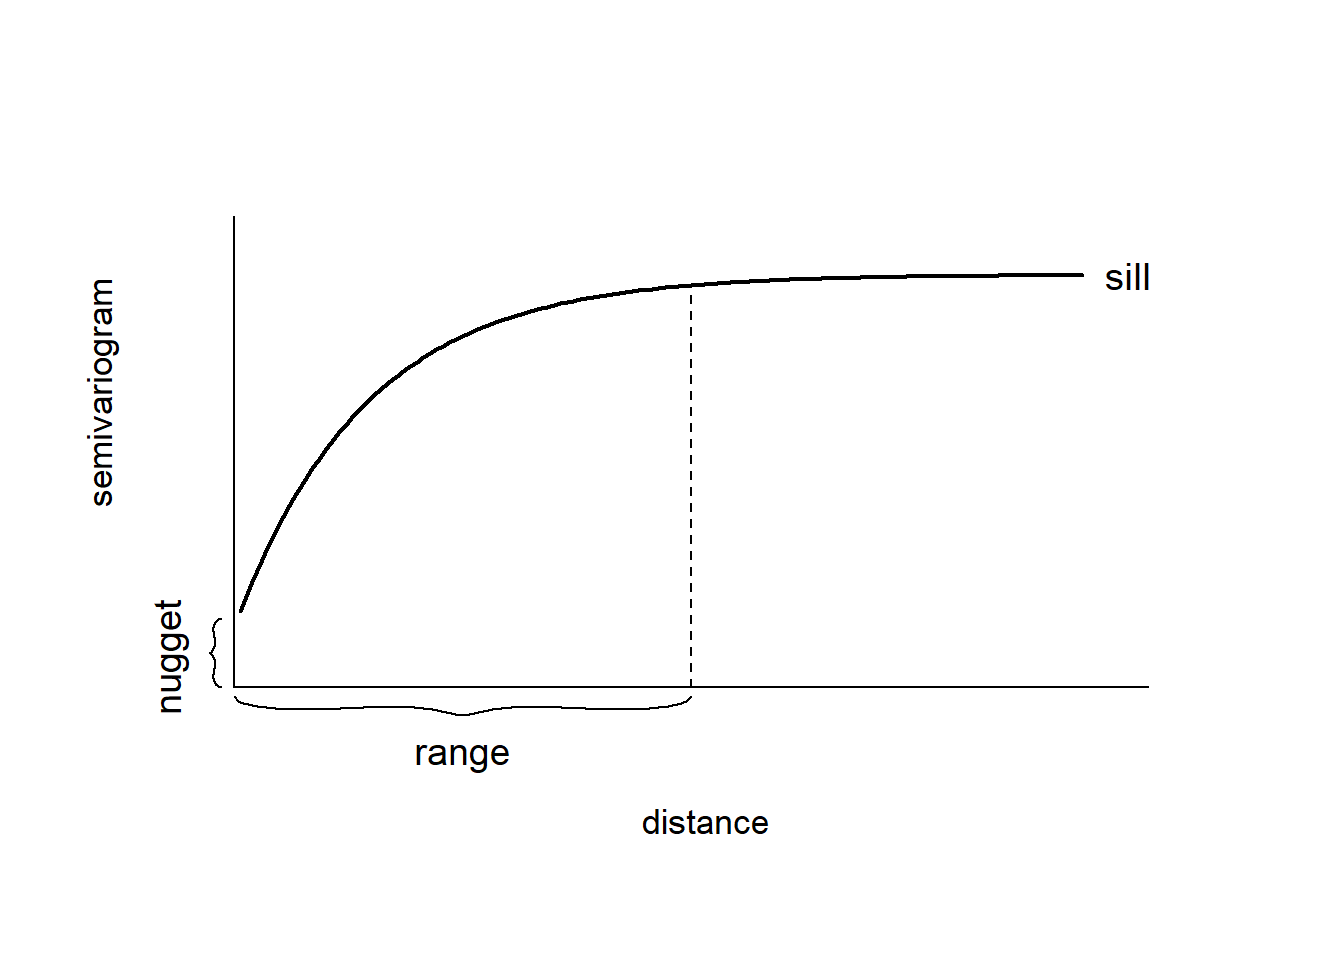
\includegraphics[width=0.85\textwidth]{typicalsemivariogram-1.png}
    \caption{A typical semivariogram}
    \label{fig:my_label}
\end{figure}
The empirical semivariogram is an exploratory tool useful for assessing whether data exhibit spatial correlation. Furthermore, it can be compared to a Monte Carlo envelope of empirical semivariograms calculated from random permutations of the data while keeping the locations fixed. If the empirical semivariogram lies outside the Monte Carlo envelope with increasing distance, this is an indication of spatial correlation.\\
The dependence structure of a GRF is given by the covariance matrix, which is constructed from a covariance function. Matérn models and exponential functions are conventionally used for this purpose. For the locations $s_i, s_j\in\mathbb{R}^2$ the exponential covariance function is given by
\begin{equation}
\hbox{Cov}\left(Z\left(s_i\right), Z\left(s_j\right)\right)=\sigma^2\exp\left(-\kappa\left|\left|s_i-s_j\right|\right|\right),
\end{equation}
where the distance between the locations $s_i$ and $s_j$ is denoted by $\left|\left|s_i-s_j\right|\right|$, the variance of the spatial field is given by $\sigma^2$, while $\kappa>0$ controls the rate at which the correlation decays as the distance increases. \\
The Matérn family represents a flexible class of covariance functions that arises naturally in a variety of scientific fields. The Matérn covariance function is written as
\begin{equation}
    \hbox{Cov}\left(Z\left(s_i\right),Z\left(s_j\right)\right)=\frac{\sigma^2}{2^{\nu-1}\Gamma\left(\nu\right)}\left(\kappa\left|\left|s_i-s_j\right|\right|\right)^{\nu}K_\nu\left(\kappa\left|\left|s_i-s_j\right|\right|\right).
\end{equation}
$\sigma^2$ denotes the marginal variance of the spatial field, $K_\nu\left(\cdot\right)$ represents the modified Bessel function of second kind and order $\nu>0$, where $\nu$ is an integer. The mean square differentiability of the process is determined by $\nu$ and is usually fixed since it is difficult to identify in applications. For $\nu=0.5$, this covariance function is the equivalent of the exponential covariance function. $\kappa > 0$ is related to the range $\rho$, which is defined as the distance at which there is approximately no correlation between two given points, $\rho=\sqrt{8\nu}/\kappa$ to be exact. Examples of these two covariance functions are shown below\autocite[Cf.][]{moraga2019geospatial}. 
\begin{figure}
    \centering
    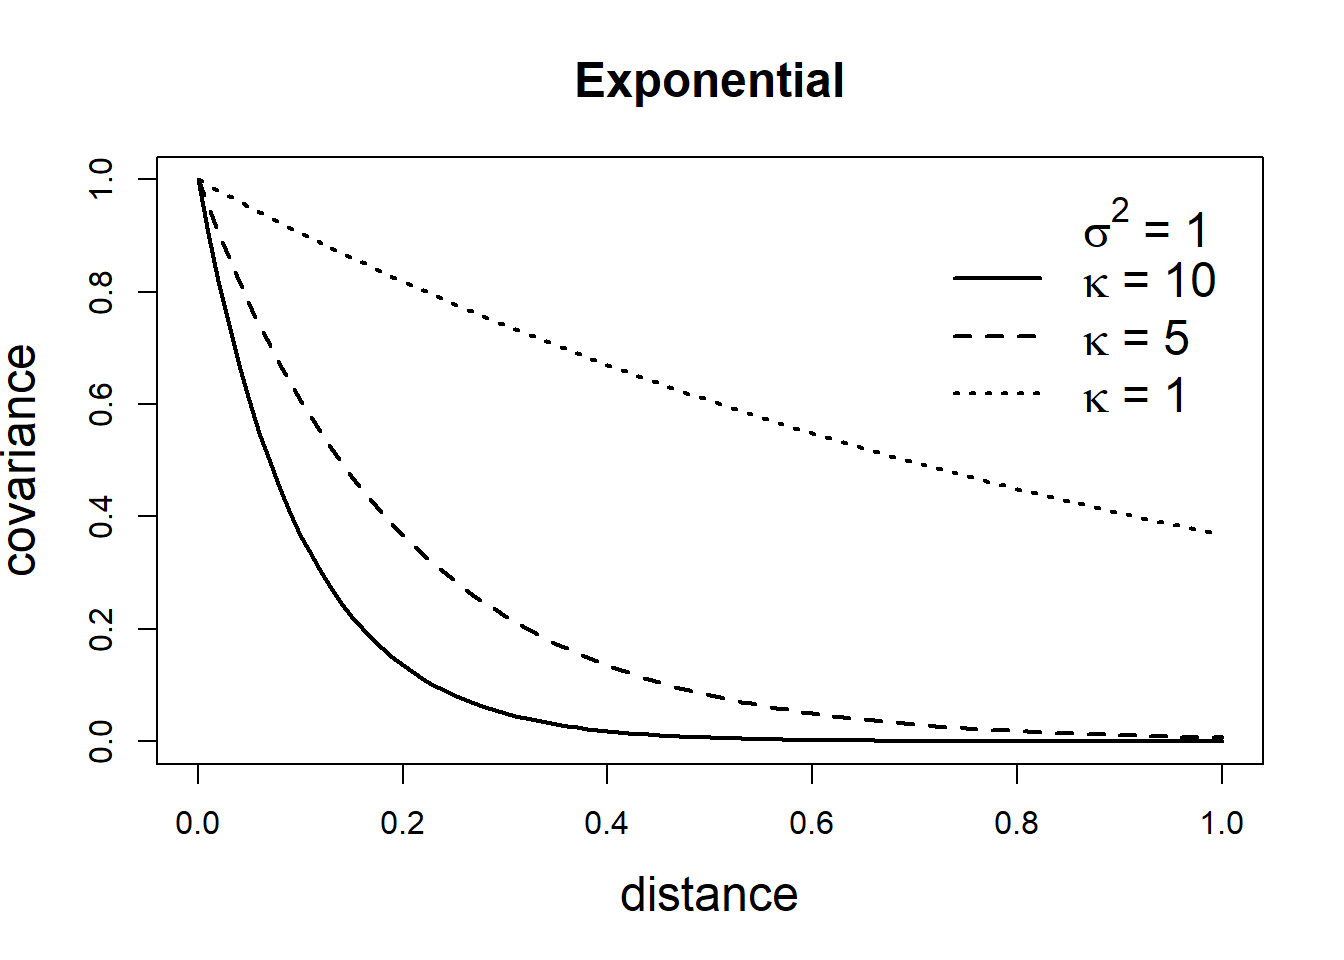
\includegraphics[width=0.8\textwidth]{covariancefunctions-1.png}
    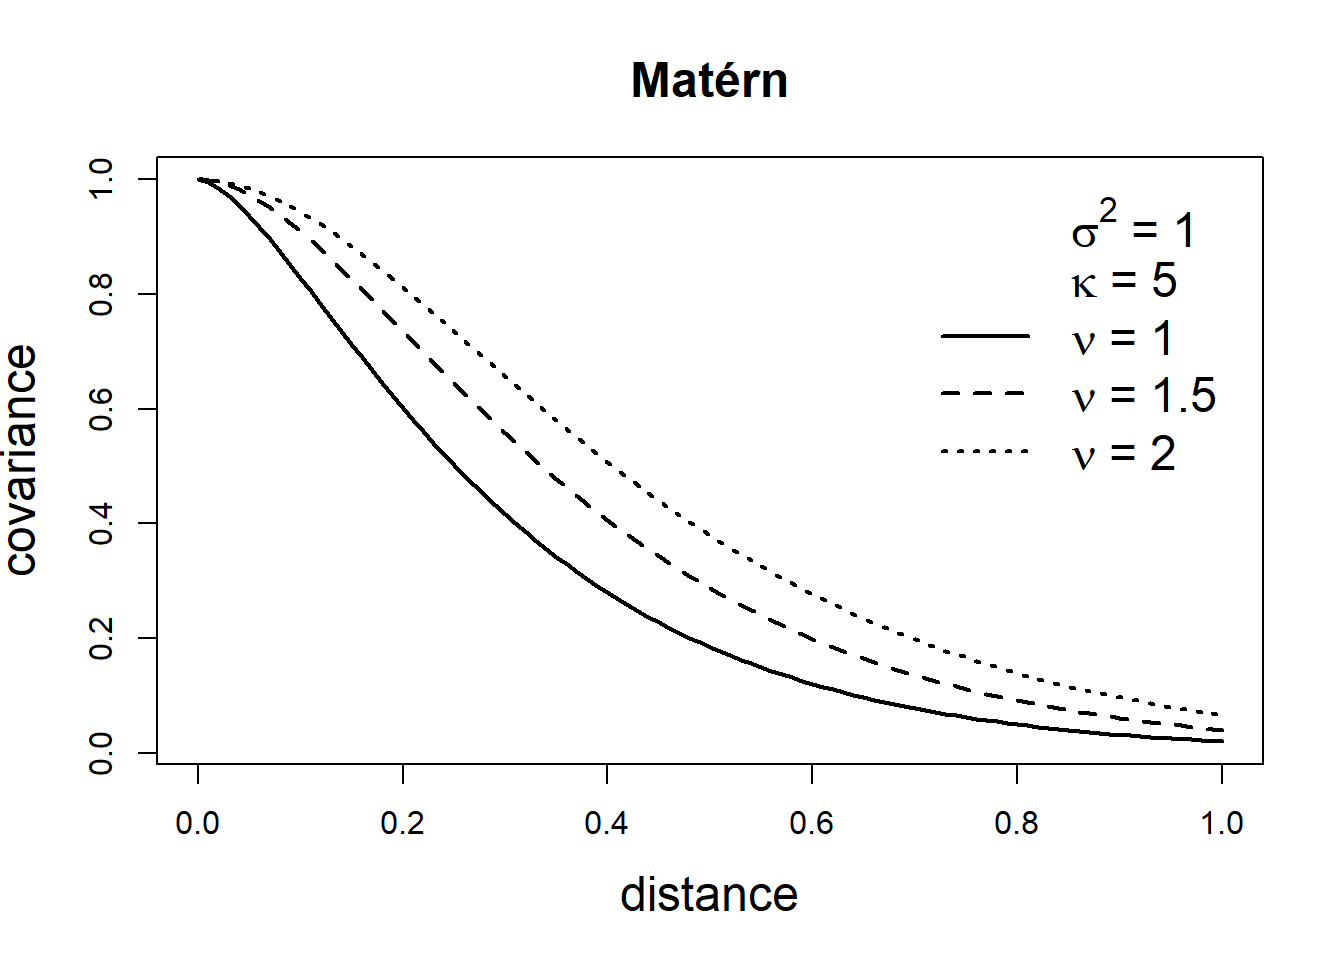
\includegraphics[width=0.8\textwidth]{covariancefunctions-2.png}
    \caption{Covariance functions corresponding to exponential and Matérn models.}
    \label{fig:covariance}
\end{figure}
\subsection{Gaussian Markov Random Fields}
\subsubsection{Definition of GMRFs}
Let $\pmb{x}=\left(x_1,...,x_n\right)^T$ be normally distributed with mean $\pmb{\mu}$ and covariance matrix $\pmb{\Sigma}$. Let $\mathcal{G}=\left(\mathcal{V}, \mathcal{E}\right)$, where $\mathcal{V}=\left\lbrace 1,...,\right\rbrace$ and $\mathcal{E}$ be such that there is no edge between nodes $i$ and $j$ exactly when $x_i\perp x_j|\pmb{x}_{ij}$. Then $\pmb{x}$ is a \textit{Gaussian Markov random field} (GMRF) with respect to $\mathcal{G}$. \\
Since $\pmb{\mu}$ does not affect the pairwise conditional independence properties of $\pmb{x}$, this information is 'hidden' in $\pmb{\Sigma}$. Hence,
\begin{equation*}
    x_i\perp x_j|x_{ij}\Longleftrightarrow Q_{ij}=0.
\end{equation*}
Therefore, the non-zero pattern of $\pmb{Q}$ determines $\mathcal{G}$, i.e. whether $x_i$ and $x_j$ are conditionally independent, and can be derived from $\pmb{Q}$. If $\pmb{Q}$ is a fully dense matrix, then $\mathcal{G}$ is fully connected, implying that any normal distribution with SPD covariance matrix is a GMRF and vice versa. \\
The elements of $\pmb{Q}$ are used for conditional interpretations. For any GMRF with respect to $\mathcal{G}=\left(\mathcal{V}, \mathcal{E}\right)$ with mean $\pmb{\mu}$ and precision matrix $\pmb{Q} > 0$,
\begin{align}
    \mathbb{E}\left[x_i|\pmb{x}_{-i}\right] &= \mu_i-\frac{1}{Q_{ii}}\sum_{j:j\sim i}Q_{ij}\left(x_j-\mu_j\right), \label{eq:mean_gmrf}\\
    \hbox{Prec}\left(x_i|\pmb{x}_{-i}\right) &= Q_{ii} \hspace{10pt}\hbox{ and }\label{eq:prec_gmrf}\\
    \hbox{Corr}\left(x_i,x_j|\pmb{x}_{ij}\right) &= -\frac{Q_{ij}}{\sqrt{Q_{ii}Q_{jj}}},\hspace{20pt} i\neq j.
\end{align}
On the main diagonal of $\pmb{Q}$ are the conditional precisions of $x_i$ given $\pmb{x}_{-i}$ are placed, while the other elements, when scaled appropriately, provide information about the conditional correlation between $x_i$ and $x_j$ given $\pmb{x}_{ij}$. Since $\hbox{Var}\left(x_i\right)=\Sigma_{ii}$ and $\hbox{Corr}\left(x_i,x_j\right)=\Sigma_{ij}/\sqrt{\Sigma_{ii}\Sigma_{jj}}$, the information about the marginal variance of $x_i$ and the marginal correlation between $x_i$ and $x_j$ is given by $\pmb{\Sigma}$. The marginal interpretation provided by the correlation matrix is intuitive and informative, as the scope of the interpretation is reduced from an $n$-dimensional distribution to a one- or two-dimensional distribution. $\pmb{Q}$ is difficult to interpret marginally because either $\pmb{x}_{-i}$ or $\pmb{x}_{ij}$ would have to be integrated out of the joint distribution parameterized with respect to $\pmb{Q}$. $\pmb{Q}^{-1}=\pmb{\Sigma}$ by definition, and in general $\Sigma_{ii}$ depends on each element in $\pmb{Q}$ and vice versa.
\subsubsection{Markov Properties of GMRFs}
One property of GMRFs is that more information regarding conditional independence can be extracted from $\mathcal{G}$. The following three properties are equivalent. \\
The \textit{pairwise Markov property}:
\begin{equation*}
    x_i\perp x_j|\pmb{x}_{ij}\hspace{20pt}\hbox{ if }\left\lbrace i,j\right\rbrace\notin\mathcal{E}\hbox{ and }i\neq j.
\end{equation*}
The \textit{local Markov property}:
\begin{equation*}
    x_i\perp \pmb{x}_{-\left\lbrace i, \hbox{ne}\left(i\right)\right\rbrace}|\pmb{x}_{\hbox{ne}\left(i\right)}\hspace{20pt}\forall i\in\mathcal{V}.
\end{equation*}
The \textit{global Markov property}:
\begin{equation*}
    \pmb{x}_{A}\perp \pmb{x}_{B}|\pmb{x}_{C}
\end{equation*}
for all disjoint sets $A$, $B$ and $C$ where $A$ and $B$ are non-empty and separated by $C$. 
\begin{figure}[H]
    \centering
    \ctikzfig{ind_fig1}
    \caption{The pairwise Markov property; the black nodes are conditionally independent given the light gray nodes.}
    \label{fig:pairwise}
\end{figure}
\begin{figure}[H]
    \centering
    \ctikzfig{ind_fig2}
    \caption{The local Markov property; the black nodes and white nodes are conditionally independent given the dark gray nodes.}
    \label{fig:local}
\end{figure}
\begin{figure}[H]
    \centering
    \ctikzfig{ind_fig3}
    \caption{The global Markov property; the dark gray and light gray nodes are globally independent given the black nodes.}
    \label{fig:global}
\end{figure}
\subsubsection{Conditional Properties of GMRFs}
An essential result of GMRFs is the conditional distribution for a subset $\pmb{x}_a$ given $\pmb{x}_{-A}$. Here the canonical parameterisation proves useful, since by definition it can be easily updated by successive conditioning. \\
By splitting the indices into the non-empty sets A and B, of which the latter is equal to -A,
\begin{equation}\label{eq:partition_1}
    \pmb{x}=\begin{pmatrix}\pmb{x}_A\\\pmb{x}_B\end{pmatrix}.
\end{equation}
The mean and the precision are divided accordingly,
\begin{equation}\label{eq:partition_2}
    \pmb{\mu}=\begin{pmatrix}\pmb{\mu}_A\\\pmb{\mu}_B\end{pmatrix},\hspace{10pt}\hbox{ and }\hspace{10pt}\pmb{Q}=\begin{pmatrix}\pmb{Q}_{AA} & \pmb{Q}_{AB} \\ \pmb{Q}_{BA} & \pmb{Q}_{BB}\end{pmatrix}.
\end{equation}
The conditional distribution of $\pmb{x}_A|\pmb{x}_B$ is then a GMRF with respect to the subgraph $\mathcal{G}^A$ with mean $\pmb{\mu}_{A|B}$ and precision matrix $\pmb{Q}_{A|B}>0$, where
\begin{equation}
    \pmb{\mu}_{A|B}=\pmb{\mu}_A-\pmb{Q}_{AA}^{-1}\pmb{Q}_{AB}\left(\pmb{x}_B-\pmb{\mu}_B\right)
\end{equation}
and
\begin{equation*}
    \pmb{Q}_{A|B}=\pmb{Q}_{AA}.
\end{equation*}
Thus, the explicit knowledge of $\pmb{Q}_{A|B}$ is available through $\pmb{Q}_{AA}$, i.e. no calculation is required to obtain the conditional precision matrix. Moreover, the conditional mean depends only on the values of $\pmb{\mu}$ and $\pmb{Q}$ in $A\cup\,\hbox{ne}\left(A\right)$, since $Q_{ij} = 0\,\forall j\not in\hbox{ne}\left(i\right)$. \\
For successive conditioning, the canonical parameterisation for GMRF is useful. \\
A GMRF $\pmb{x}$ with respect to $\mathcal{G}$ and canonical parameters $\pmb{b}$ and $\pmb{Q}>0$ has the density
\begin{equation*}
    \pi\left(\pmb{x}\right)\propto\exp\left(-1\frac{1}{2}\pmb{x}^T\pmb{Q}\pmb{x}+\pmb{b}^T\pmb{x}\right).
\end{equation*}
The precision matrix is $\pmb{Q}$ and the mean is $\pmb{\mu}=\pmb{Q}^{-1}\pmb{b}$. The canonical parameterisation is written as 
\begin{equation*}
    \pmb{x}\sim \mathcal{N}_C\left(\pmb{b},\pmb{Q}\right).
\end{equation*}
Furthermore,
\begin{equation*}
    \mathcal{N}\left(\pmb{\mu},\pmb{Q}^{-1}\right) \Longleftrightarrow \mathcal{N}_C\left(\pmb{Q\mu}, \pmb{Q}\right).
\end{equation*}
If the indices are partitioned into two non-empty sets A and B and $\pmb{x}$, $\pmb{b}$ and $\pmb{Q}$ are partitioned as in \eqref{eq:partition_1} and \eqref{eq:partition_2}, then
\begin{equation}
    \pmb{x}_A|\pmb{x}_B\sim\mathcal{N}_C\left(\pmb{b}_A-\pmb{Q}_{AB}\pmb{x}_B,\pmb{Q}_{AA}\right).
\end{equation}
Let $\pmb{y}|\pmb{x}\sim\mathcal{N}\left(\pmb{x},\pmb{P}^{-1}\right)$ and $\pmb{x}\sim\mathcal{N}_C\left(\pmb{b},\pmb{Q}\right)$, then
\begin{equation}
    \pmb{x}|\pmb{y}\sim\mathcal{N}_C\left(\pmb{b}+\pmb{Py}, \pmb{Q}+\pmb{P}\right).
\end{equation}
This allows the calculation of conditional densities with multiple sources of conditioning, e.g. conditioning on observed data and a subset of variables. Therefore, the canonical parameterisation can be repeatedly updated without explicitly calculating the mean until it is actually needed. The computation of the mean requires the solution of $\pmb{Q\mu}=\pmb{b}$, but only matrix-vector products are needed for updating the canonical parameterisation.
\subsubsection{Specification Through Full Conditionals}
Alternatively, a GMRF can be specified by the full conditionals $\left\lbrace\pi\left(x_i|\pmb{x}_{-i}\right)\right\rbrace$ in place of $\pmb{\mu}$ and $\pmb{Q}$. Suppose the full conditionals are given as normals with
\begin{align}
    \mathbb{E}\left[x_i|\pmb{x}_{-i}\right] &= \mu_i-\sum_{j:j\sim i}\beta_{ij}\left(x_j-\mu_j\right)\hspace{10pt}\hbox{ and}\\
    \hbox{Prec}\left(x_i|\pmb{x}_{-i}\right) &= \kappa_i>0
\end{align}
for $i=1,...,n$, for $\pmb{\mu}$, $\pmb{\kappa}$ and some $\left\lbrace\eta_{ij},i\neq j\right\rbrace$. Evidently, $\sim$ is implicitly defined by the non-zero terms of $\left\lbrace\beta_{ij}\right\rbrace$. For there to exist a joint density $\pi\left(\pmb{x}\right)$ leading to these full conditional distributions, these full conditionals must be consistent. Since $\sim$ is symmetric, it follows that if $\beta_{ij}\neq 0$, then $\beta_{ji}\neq0$. If the entries of the precision matrix are chosen such that
\begin{equation*}
    Q_{ii}=\kappa_i, \hspace{10pt}\hbox{ and }\hspace{10pt} Q_{ij}=\kappa_i\beta_{ij}
\end{equation*}
and $\pmb{Q}$ must be symmetrical, i.e.,
\begin{equation*}
    \kappa_i\beta_{ij}=\kappa_j\beta_{ji},
\end{equation*}
then $\pmb{x}$ is a GMRF with respect to a labelled graph $\mathcal{G}=\left(\mathcal{V}, \mathcal{E}\right)$ with mean $\pmb{\mu}$ and precision matrix $\pmb{Q}=\left(Q_{ij}\right)$.
\subsubsection{Multivariate GMRFs}
A \textit{multivariate GMRF} (MGMRF) is a multivariate extension of a GMRF that has proven useful in applications. Let $\pmb{x}$ be a GMRF with respect to $\mathcal{G}$, then the Markov property implies that
\begin{equation*}
    \pi\left(x_i|\pmb{x}_{-i}\right)=\pi\left(x_i|\left\lbrace x_j:j\sim i\right\rbrace\right).
\end{equation*}
$x_i$ is the value related to node $i$. Often the nodes have physical interpretations such as an administrative region of a country, which can be used to define the neighbours of node $i$. Let each of the $n$ nodes have an associated vector $\pmb{x}_i$ of dimension $p$, resulting in a GMRF of size $np$. Such a GMRF is denoted by $\pmb{x}=\left(\pmb{x}_1^T,...,\pmb{x}_n^T\right)^T$. The Markov property with respect to the nodes is preserved, i.e.,
\begin{equation*}
    \pi\left(\pmb{x}_i|\pmb{x}_{-i}\right)=\pi\left(\pmb{x}_i|\left\lbrace\pmb{x}_{j}:j\sim i\right\rbrace\right),
\end{equation*}
where $\sim$ is with respect to \textit{the same graph} $\mathcal{G}$. Let $\pmb{\mu}=\left(\pmb{\mu}_1^T,... ,\pmb{\mu}_n^T\right)^T$ be the mean of $\pmb{x}$, where $\mathbb{E}\left[\pmb{x}_i\right]=\pmb{\mu}_i$, and $\widetilde{\pmb{Q}}=\left(\widetilde{\pmb{Q}}_{ij}\right)$ its precision matrix, where each element of the matrix is a $p\times p$ matrix. \\
It follows that
\begin{equation*}
    \pmb{x}_i\perp\pmb{x}_j|\pmb{x}_{-ij}\Longleftrightarrow\widetilde{\pmb{Q}}_{ij}=\pmb{0}.
\end{equation*}
Formally, a random vector $\pmb{x}=\left(\pmb{x}_1^T,...,\pmb{x}_n^T\right)^T$ with $\dim\left(\pmb{x}_i\right)=p$, is called a $\hbox{MGMRF}_p$ with respect to $\mathcal{G}=\left(\mathcal{V}=\left\lbrace 1,. ...,n\right\rbrace,\mathcal{E}\right)$ with mean $\pmb{\mu}$ and precision matrix $\widetilde{\pmb{Q}} >0$, exactly when its density has the form
\begin{align*}
    \pi\left(\pmb{x}\right) &=\left(\frac{1}{2\pi}\right)^{np/2}\left|\widetilde{\pmb{Q}}\right|^{1/2}\exp\left(-\frac{1}{2}\left(\pmb{x}-\pmb{\mu}\right)^T\widetilde{\pmb{Q}}\left(\pmb{x}-\pmb{\mu}\right)\right)\\
    &=\left(\frac{1}{2}\right)^{np/2}\left|\widetilde{\pmb{Q}}\right|^{1/2}\exp\left(-\frac{1}{2}\sum_{ij}\left(\pmb{x}_i-\pmb{\mu}_i\right)^T\widetilde{\pmb{Q}}_{ij}\left(\pmb{x}_j-\pmb{\mu}_j\right)\right)
\end{align*}
and
\begin{equation*}
    \widetilde{\pmb{Q}}_{ij}\neq0\Longleftrightarrow\left\lbrace i,j\right\rbrace\in\mathcal{E}\,\forall\,i\neq j.
\end{equation*}
A $\hbox{MGMRF}_p$ is equivalent to a GMRF of dimension $np$ with identical mean vector and precision matrix.  Therefore, all results valid for a GMRF are also valid for a $\hbox{MGMRF}_p$, with modifications, since the graph for a $\hbox{MGMRF}_p$ has size $n$ and is defined with respect to $\left\lbrace\pmb{x}_i\right\rbrace$, while for a GMRF it has size $np$ and is defined with respect to $\left\lbrace x_i\right\rbrace$.  \\
The interpretation of $\widetilde{\pmb{Q}}_{ii}$ and $\widetilde{\pmb{Q}}_{ij}$ can be derived from the full conditional $\pi\left(\pmb{x}_i|\pmb{x}_{-i}\right)$. The extensions of \eqref{eq:mean_gmrf} and \eqref{eq:prec_gmrf} are
\begin{align}
    \mathbb{E}\left[\pmb{x}_i|\pmb{x}_{-i}\right]&=\pmb{\mu}_i-\widetilde{\pmb{Q}}_{ii}^{-1}\sum_{j:j\sim i}\widetilde{\pmb{Q}}_{ij}\left(\pmb{x}_j-\pmb{\mu}_j\right)\\
    \hbox{Prec}\left(\pmb{x}_i|\pmb{x}_{-i}\right) &= \widetilde{\pmb{Q}}_{ii}.
\end{align}
In some applications, the full conditionals
\begin{align}
    \mathbb{E}\left[\pmb{x}_i|\pmb{x}_{-i}\right] &= \pmb{\mu}_i-\sum_{j:j\sim i}\pmb{\beta}_{ij}\left(\pmb{x}_j-\pmb{\mu}_j\right) \\
    \hbox{Prec}\left(\pmb{x}_i|\pmb{x}_{-i}\right) &= \pmb{\kappa}_i > 0,
\end{align}
In some applications, the full conditionals are used to define the $\hbox{MGMRF}_p$, for given $p\times p$-matrices $\left\lbrace\pmb{\beta}_{ij},i\neq j\right\rbrace$, $\left\lbrace\pmb{\kappa}_i\right\rbrace$, and vectors $\pmb{\mu}_i$. Again, $\sim$ is implicitly defined by the non-zero matrices $\left\lbrace\pmb{\kappa}_i\right\rbrace$. Similar requirements as for $p=1$ apply to the existence of the joint density: $\pmb{\kappa}_i\pmb{\beta}_{ij}=\pmb{\beta}_{ij}^T\pmb{\kappa}_j$ for $i\neq j$ and $\widetilde{\pmb{Q}} > 0$. The $p\times p$ elements of $\widetilde{\pmb{Q}}$ are
\begin{equation*}
    \widetilde{\pmb{Q}}_{ij}=\begin{cases}
    \pmb{\kappa}_i\pmb{\beta}_{ij} & i\neq j \\
    \pmb{\kappa}_i & i=j
    \end{cases};
\end{equation*}
therefore $\widetilde{\pmb{Q}}>0\Longleftrightarrow\left(\pmb{I}+\left(\pmb{\beta}_{ij}\right)\right) > 0$\autocite[Cf.][]{rue2005gaussian}.
\subsection{Integrated Nested Laplace Approximation}
An alternative to MCMC methods that is both less computationally intensive and suitable for performing approximate Bayesian inference in latent Gaussian models is \textit{Integrated nested Laplace Approximation} (INLA). The basis of INLA is the use of a combination of analytical approximations and numerical algorithms for sparse matrices to approximate the posterior distribution using closed-form expressions. This speeds up inference and circumvents problems of sample convergence and mixing, making it suitable for fitting large data sets or exploring other models.  \\
INLA can be used for all models of the following form,
\begin{align*}
    y_i|\pmb{x},\pmb{\theta} &\sim \pi\left(y_i|x_i,\pmb{\theta}\right), \hspace{20pt} i=1,...,n,\\
    \pmb{x}|\pmb{\theta} &\sim \mathcal{N}\left(\mu\left(\pmb{\theta}\right), \pmb{Q}\left(\pmb{\theta}\right)^{-1}\right), \\
    \pmb{\theta} &\sim \pi\left(\pmb{\theta}\right).
\end{align*}
As introduced in \autoref{sec:notation}, $\pmb{y}$ are the observed data, $\pmb{x}$ is a Gaussian field, $\pmb{\theta}$ represents the hyperparameters, while $\mu\left(\pmb{\theta}\right)$ and $\pmb{Q}\left(\pmb{\theta}\right)$ denote the mean and precision matrix respectively.To ensure fast inference, the dimension of the hyperparameter vector $\pmb{\theta}$ should be small, since the approximations are computed by numerical integration over the hyperparameter space. \\
In most cases, the observations $y_i$ are assumed to belong to the exponential family with mean $\mu_i=g^{-1}\left(\eta_i\right)$. As shown in equation \eqref{eq:predictor}, $\eta_i$ accounts for the effects of several covariates in an additive way, which makes it suitable for a wide range of models, including spatial and spatio-temporal models, since $\left\lbrace f^{(j)}\right\rbrace$ can take very different forms. \\
Let $\pmb{x}=\left(\alpha,\left\lbrace\beta_k\right\rbrace|\theta\sim\mathcal{N}\left(\mu\left(\theta\right), \pmb{Q}\left(\theta\right)^{-1}\right)\right)$ be the vector of latent Gaussian variables, and let $\pmb{\theta}$ be the vector of hyperparameters, which are not required to be Gaussian. INLA calculates accurate and fast approximations for the posterior marginals of the components of the latent Gaussian variables
\begin{equation*}
    \pi\left(x_i|\pmb{y}\right),\hspace{20pt}i=1,...,n,
\end{equation*}
as well as the posterior marginals for the hyperparameters of the latent Gaussian model
\begin{equation*}
    \pi\left(\theta_j|\pmb{y}\right),\hspace{20pt}j=1,...,\dim\left(\pmb{\theta}\right).
\end{equation*}
For each element $x_i$ of $\pmb{x}$ the posterior marginals are given by
\begin{equation}
    \pi\left(x_i|\pmb{y}\right)=\int\pi\left(x_i|\pmb{\theta},\pmb{y}\right)\pi\left(\pmb{\theta}|\pmb{y}\right)d\pmb{\theta},
\end{equation}
and the posterior marginal for the hyperparameters can be expressed by
\begin{equation}
    \pi\left(\theta_j|\pmb{y}\right)=\int\pi\left(\pmb{\theta}|\pmb{y}\right)d\pmb{\theta}_{-j}.
\end{equation}
$\pi\left(x_i|\pmb{y}\right)$ is approximated by combining analytical approximations to the full conditionals $\pi\left(x_i|\pmb{\theta},\pmb{y}\right)$ and $\pi\left(\pmb{\theta}|\pmb{y}\right)$ and numerical integration routines to integrate out $\pmb{\theta}$. Similarly, $\pi\left(\theta_j|\pmb{y}\right)$ is approximated by approximating $\pi\left(\pmb{\theta}|\pmb{y}\right)$ and integrating out $\pmb{\theta}_{-j}$. In particular, the posterior density of $\pmb{\theta}$ is obtained through Gaussian approximation for the posterior of the latent field, $\widetilde{\pi}_G\left(\pmb{x}|\pmb{\theta},\pmb{y}\right)$, evaluated at the posterior mode, $x^*\left(\pmb{\theta}\right)=\arg\max_{\pmb{x}}\pi_G\left(\pmb{x}|\pmb{\theta},\pmb{y}\right)$,
\begin{equation}
    \widetilde{\pi}\left(\pmb{\theta}|\pmb{y}\right)\propto\frac{\pi\left(\pmb{x},\pmb{\theta},\pmb{y}\right)}{\widetilde{\pi}_G\left(\pmb{x}|\pmb{\theta},\pmb{y}\right)}\bigg|_{\pmb{x}=x^*\left(\pmb{\theta}\right)}.
\end{equation}
Next, the following nested approximations are constructed,
\begin{equation}
    \widetilde{\pi}\left(x_i|\pmb{y}\right)=\int\widetilde{\pi}\left(x_i|\pmb{\theta},\pmb{y}\right)\widetilde{\pi}\left(\pmb{\theta}|\pmb{y}\right)d\pmb{\theta},\hspace{20pt}\widetilde{\pi}\left(\theta_j|\pmb{y}\right)=\int\widetilde{\pi}\left(\pmb{\theta}|\pmb{y}\right)d\pmb{\theta}_{-j}.
\end{equation}
Finally, these approximations are numerically integrated with respect to $\pmb{\theta}$
\begin{align}
    \widetilde{\pi}\left(x_i|\pmb{y}\right)&=\sum_k\widetilde{\pi}\left(x_i|\theta_k,\pmb{y}\right)\widetilde{\pi}\left(\theta_k|\pmb{y}\right)\times\Delta_k,\\
    \widetilde{\pi}\left(\theta_j|\pmb{y}\right)&=\sum_l\widetilde{\pi}\left(\theta_l^*|\pmb{y}\right)\times\Delta_l^*,
\end{align}
with $\Delta_k$ and $\Delta_l^*$ representing the area weights corresponding to $\theta_k$ and $\theta_l^*$. \\
To obtain the approximations for the posterior marginals for the $x_i$'s conditioned on selected values of $\theta_k$ and $\widetilde{\pi}\left(x_i|\theta_k,\pmb{y}\right)$, a Gaussian, Laplace or simplified Laplace approximation can be used. Using a Gaussian approximation derived from $\widetilde{\pi}_G\left(\pmb{x}|\pmb{\theta},\pmb{y}\right)$ is the simplest and fastest solution, but in some situations it produces errors in the location and is unable to capture skewness behaviour. Therefore, the Laplace approximation is favoured over the Gaussian approximation, although it is relatively expensive. The simplified Laplace approximation is associated with lower costs and addresses inaccuracies of the Gauss approximation in terms of location and skewness in a satisfactory manner\autocite[Cf.][]{moraga2019geospatial}.
%https://arxiv.org/pdf/1708.02723.pdf \\
%http://www.leg.ufpr.br/~elias/cursos/br2019/slides1.pdf